\documentclass[11pt]{article}

\usepackage[a4paper,margin=1in]{geometry}
\usepackage{amsmath,amssymb,bm,mathtools}
\usepackage{booktabs}
\usepackage{float}
\usepackage{graphicx}
\usepackage{hyperref}
\usepackage{microtype}

\hypersetup{
  colorlinks=true,
  linkcolor=blue,
  citecolor=blue,
  urlcolor=blue
}

\newcommand{\ii}{\mathrm{i}}
\newcommand{\dd}{\mathrm{d}}
\newcommand{\bfa}{\bm{a}}
\newcommand{\bfb}{\bm{b}}
\newcommand{\bff}{\bm{f}}
\newcommand{\bfu}{\bm{u}}
\newcommand{\bfv}{\bm{v}}
\newcommand{\bfq}{\bm{q}}
\newcommand{\bfzero}{\bm{0}}
\newcommand{\Graw}{G_{\mathrm{raw}}}
\newcommand{\Gdiv}{G_{\mathrm{div}}}
\newcommand{\Gbdry}{G_{\partial}}
\newcommand{\Gtilde}{\widetilde{G}}
\newcommand{\Ez}{E_z}
\newcommand{\Ex}{E_x}
\newcommand{\Ey}{E_y}
\newcommand{\Dz}{D_z}
\newcommand{\Bbdry}{B_{\partial}}
\newcommand{\Bzero}{B_{0,\mathrm{DNS}}}
\newcommand{\Badm}{B_{\mathrm{adm},\mathrm{DNS}}}
\newcommand{\Pmat}{P}

\title{Numerical sampling and constraint construction for a Chebyshev-Fourier DNS of turbulent channel flow}
\author{Prepared for the MKM channel-flow data-estimation workflow}
\date{\today}

\begin{document}

\maketitle

\begin{abstract}
This note gives a self-contained description of the numerical setup used to
sample data from the MKM channel-flow demonstration in \texttt{shenfun}, and of
the postprocessing procedure used to construct the target quantities for a
horizontally periodic, wall-normal inhomogeneous data set. The discussion is
organized at the level needed to reproduce the stored objects in the HDF5
target file. We first define the channel-flow geometry, the Chebyshev-Fourier
mesh, the two-stage spin-up and sampling procedure, and the component ordering
used by the stored data. We then derive, step by step, the sampled mean
profile, Reynolds-stress profile, horizontal Fourier coefficients, equal-time
modal covariance, positive-lag modal covariance, and plane-averaged temporal
auto-covariance and auto-spectrum diagnostics. The production two-stage run on
the current \((N_x,N_y,N_z)=(64,32,64)\) mesh is then summarized, including
the accepted sampling window, block-convergence checks, instantaneous and mean
velocity contours, mean velocity profile, Reynolds-stress tensor profile,
temporal diagnostics, and constraint audit. Finally, we derive the modewise
incompressibility and no-slip
constraint matrix on the solver-native Chebyshev-Gauss quadrature grid,
including the barycentric spectral derivative, the endpoint interpolation
boundary operator, and the singular-value compression used to obtain the saved
row-orthonormal constraint \(\Gtilde(\kappa,\lambda)\).
\end{abstract}

\noindent\textbf{Keywords:}
channel flow; direct numerical simulation; Chebyshev-Fourier method; modal
covariance; incompressibility constraint; barycentric interpolation.

\section{Purpose and scope}

The objective of the workflow described here is to collect and postprocess a
direct numerical simulation (DNS) of plane channel flow into a target data
layout suitable for horizontally periodic, wall-normal inhomogeneous modeling.
The DNS is run using the MKM channel-flow demonstration provided by
\texttt{shenfun}. The postprocessed data are stored in horizontal Fourier space
and retain the wall-normal dependence explicitly. For each horizontal mode, the
stored quantities are compatible with a discrete incompressibility and no-slip
constraint matrix.

This note focuses on the numerical method and the exact objects generated by
the scripts in
\[
  \texttt{scripts/mkm\_dns\_target}.
\]
The current production data set is generated by a two-stage run. A first stage
develops the flow from the MKM demonstration initialization and writes no
target snapshots. A second stage restarts from the accepted checkpoint and
writes the velocity snapshots used for statistics and covariance estimation.
The short four-snapshot run used earlier to validate the mechanics of this
workflow is superseded here by the production run described in
Section~\ref{sec:production_results}.

\section{Physical and numerical setup}

\subsection{Channel geometry and variables}

Let \(x\in[0,L_x)\) denote the streamwise coordinate, let \(y\in[0,L_y)\)
denote the spanwise coordinate, and let \(z\in[-1,1]\) denote the wall-normal
coordinate. The considered channel has
\[
  L_x = 2\pi,\qquad L_y=\pi.
\]
The velocity is written in the target component order
\[
  \bfu = (u_x,u_y,u_z)^T,
\]
where \(u_x\) is streamwise velocity, \(u_y\) is spanwise velocity, and \(u_z\)
is wall-normal velocity. In these variables the incompressibility constraint is
\begin{equation}
  \partial_x u_x + \partial_y u_y + \partial_z u_z = 0.
  \label{eq:continuous_divergence}
\end{equation}
The no-slip condition at both walls is
\begin{equation}
  \bfu(x,y,-1,t)=\bfzero,\qquad \bfu(x,y,1,t)=\bfzero.
  \label{eq:continuous_noslip}
\end{equation}

The solver advances the incompressible Navier-Stokes equations in a
constant-flux channel configuration at friction Reynolds number
\[
  Re_{\tau}=180.
\]
In nondimensional form, a representative statement of the equation being
advanced is
\begin{align}
  \nabla\cdot\bfu &= 0, \label{eq:ns_div}\\
  \partial_t\bfu + \bfu\cdot\nabla\bfu
    &= -\nabla p + \frac{1}{Re_{\tau}}\Delta\bfu + f_x(t)\bm{e}_x,
    \label{eq:ns_momentum}
\end{align}
with periodicity in \(x\) and \(y\) and no-slip walls in \(z\). The MKM
implementation uses the Kim-Moin-Moser channel-flow formulation in which the
wall-normal velocity and wall-normal vorticity are advanced spectrally, while
the remaining velocity components are reconstructed from incompressibility and
the zero-horizontal-wavenumber momentum equations. This note does not require
the internal solver variables; the sampled and constrained objects are written
in the physical velocity component order \((u_x,u_y,u_z)\).

\subsection{Nondimensionalization used in the figures}

The natural scales for the present channel-flow data are the channel
half-height \(h\) and the friction velocity \(u_{\tau}\). In the MKM
configuration used here,
\[
  h=\frac{1-(-1)}{2}=1,\qquad u_{\tau}=1,\qquad
  \nu=\frac{u_{\tau}h}{Re_{\tau}}=\frac{1}{180}.
\]
All figures below therefore report the nondimensional coordinates and
statistics
\begin{equation}
  x^*=\frac{x}{h},\qquad y^*=\frac{y}{h},\qquad
  z^*=\frac{z}{h},\qquad t^*=\frac{t u_{\tau}}{h},
  \label{eq:plot_coordinate_scales}
\end{equation}
and
\begin{equation}
  u_i^*=\frac{u_i}{u_{\tau}},\qquad
  R_{\alpha\beta}^*=\frac{R_{\alpha\beta}}{u_{\tau}^2}.
  \label{eq:plot_value_scales}
\end{equation}
Since \(h=u_{\tau}=1\) in this run, these scalings leave the numerical values
unchanged, but they identify the axes and colorbar values as friction-scaled
channel-flow quantities. The constant-flux diagnostic gives the reference bulk
velocity
\begin{equation}
  \frac{U_b}{u_{\tau}}
  =
  \frac{Q}{2hL_xL_yu_{\tau}}
  \approx
  \frac{618.9703}{4\pi^2}
  =
  15.6788,
  \label{eq:bulk_velocity_reference}
\end{equation}
which is useful as a run check but is not used as the primary plotting scale;
the velocity and Reynolds-stress plots use the standard friction scaling in
Eqs.~\eqref{eq:plot_coordinate_scales}--\eqref{eq:plot_value_scales}.

\subsection{Chebyshev-Fourier grid}

The current mesh is
\[
  (N_x,N_y,N_z) = (64,32,64),
\]
where \(N_x\) is the number of streamwise points, \(N_y\) is the number of
spanwise points, and \(N_z\) is the number of wall-normal quadrature points.

The default saved wall-normal mesh is the solver-native Chebyshev-Gauss
quadrature mesh. For a general interval \([a,b]\), the nodes are
\begin{equation}
  z_m = \frac{a+b}{2} + \frac{b-a}{2}
        \cos\left(\frac{(2m+1)\pi}{2N_z}\right),
  \qquad m=0,\ldots,N_z-1.
  \label{eq:cheb_gauss_nodes}
\end{equation}
For the present channel \(a=-1\) and \(b=1\). The endpoints \(z=-1\) and
\(z=1\) are not members of the Chebyshev-Gauss grid; this point matters for
the construction of the boundary rows in Section~\ref{sec:constraint}.

The horizontal grids are equispaced:
\begin{equation}
  x_j = j\frac{L_x}{N_x},\qquad j=0,\ldots,N_x-1,
  \label{eq:x_grid}
\end{equation}
and
\begin{equation}
  y_\ell = \ell\frac{L_y}{N_y},\qquad \ell=0,\ldots,N_y-1.
  \label{eq:y_grid}
\end{equation}
The corresponding discrete Fourier wavenumbers are those returned by
\(\texttt{numpy.fft.fftfreq}\):
\begin{align}
  \kappa_p &= 2\pi\,\mathrm{fftfreq}(N_x,L_x/N_x)_p,
  &&p=0,\ldots,N_x-1, \label{eq:kappa_grid}\\
  \lambda_q &= 2\pi\,\mathrm{fftfreq}(N_y,L_y/N_y)_q,
  &&q=0,\ldots,N_y-1. \label{eq:lambda_grid}
\end{align}

\subsection{Time integration and staged sampling}

The production run used the following solver settings:
\[
\begin{gathered}
  Re_{\tau}=180,\qquad \Delta t=5\times 10^{-4},\qquad
  \texttt{conv}=0,\\
  \texttt{family}=\texttt{C},\qquad
  \texttt{padding\_factor}=(1.5,1.5,1.5),\qquad
  \texttt{timestepper}=\texttt{IMEXRK222}.
\end{gathered}
\]
The data collection is explicitly split into two stages.

First, a spin-up stage starts from the MKM demonstration initialization. It
writes no velocity snapshots for the target data set. Its only persistent
state is a checkpoint forced at the final time. In the production run,
\[
  t_{\mathrm{spin}}u_{\tau}/h = 20,\qquad n_{\mathrm{spin}}=40000.
\]

Second, a sampling stage restarts from this checkpoint and writes velocity
snapshots at a fixed step cadence. Snapshots were written every
200 time steps, so that
\[
  \Delta t_{\mathrm{sample}} u_{\tau}/h = 200\Delta t\,u_{\tau}/h = 0.1.
\]
The sampling stage was appended in four segments:
\[
  [20,60],\qquad [60,100],\qquad [100,140],\qquad [140,180].
\]
The first segment created the sampled velocity file, and the later segments
used append mode. The raw sampled velocity file therefore covers
\[
  t u_{\tau}/h=20.1,\;20.2,\ldots,180.0,
\]
with \(1600\) snapshots. No spin-up snapshots are present in that sampled
velocity file. After convergence checks, the accepted target window was chosen
as
\begin{equation}
  \mathcal{T}_{\mathrm{acc}} = \{60.0,60.1,\ldots,180.0\}
  \quad\text{in }t u_{\tau}/h,
  \qquad N_s=1201.
  \label{eq:accepted_sample_times}
\end{equation}
Only these accepted snapshots enter the final mean, Reynolds-stress, modal
coefficient, and covariance estimates.

\section{Sampled velocity fields and target statistics}
\label{sec:sampled_outputs}

\subsection{Component ordering}

The MKM HDF5 output groups use the solver component labels
\[
  \texttt{u0}=u_z,\qquad
  \texttt{u1}=u_x,\qquad
  \texttt{u2}=u_y.
\]
The postprocessor reorders these into the target component order
\[
  (u_x,u_y,u_z).
\]
Let \(\alpha,\beta\in\{x,y,z\}\) denote target component indices. For the
\(n\)-th selected snapshot, define the sampled velocity values
\[
  u_\alpha(x_j,y_\ell,z_m,t_n),
  \qquad n=0,\ldots,N_s-1,
\]
where \(N_s\) is the number of selected snapshots. Unless otherwise stated,
the time origin in the estimators is reset to the first retained snapshot, so
\[
  t_n=n\Delta t_s .
\]
The accepted production target uses \(N_s=1201\).

\subsection{Mean profile}

Because the channel is statistically homogeneous in \(x\) and \(y\), the mean
profile is a function only of the wall-normal coordinate. The estimator used in
the target file is the average over selected snapshots and both horizontal
directions:
\begin{equation}
  \overline{u}_{\alpha}(z_m)
  =
  \frac{1}{N_sN_xN_y}
  \sum_{n=0}^{N_s-1}
  \sum_{j=0}^{N_x-1}
  \sum_{\ell=0}^{N_y-1}
  u_\alpha(x_j,y_\ell,z_m,t_n).
  \label{eq:mean_profile}
\end{equation}
This is the dataset \(\texttt{mean\_profile}\), stored with shape
\[
  (N_z,3).
\]

\subsection{Fluctuation field}

The fluctuation field is formed by subtracting the estimated mean profile from
each selected snapshot:
\begin{equation}
  u'_\alpha(x_j,y_\ell,z_m,t_n)
  =
  u_\alpha(x_j,y_\ell,z_m,t_n)
  -
  \overline{u}_{\alpha}(z_m).
  \label{eq:fluctuation}
\end{equation}
This definition ensures that the horizontal and snapshot average of
\(u_\alpha'\) is zero for each wall-normal level when the same selected
snapshots are used in Eqs.~\eqref{eq:mean_profile} and
\eqref{eq:fluctuation}.

\subsection{Reynolds-stress profile}

The stored Reynolds-stress profile is the second moment of the fluctuation
field at each wall-normal level:
\begin{equation}
  R_{\alpha\beta}(z_m)
  =
  \frac{1}{N_sN_xN_y}
  \sum_{n=0}^{N_s-1}
  \sum_{j=0}^{N_x-1}
  \sum_{\ell=0}^{N_y-1}
  u'_\alpha(x_j,y_\ell,z_m,t_n)
  u'_\beta(x_j,y_\ell,z_m,t_n).
  \label{eq:reynolds}
\end{equation}
The stored dataset is \(\texttt{reynolds\_stress\_profile}\), with shape
\[
  (N_z,3,3).
\]

\subsection{Horizontal Fourier coefficients}

For each snapshot and wall-normal level, the horizontal Fourier coefficient of
the fluctuation field is defined by the normalized two-dimensional discrete
Fourier transform
\begin{equation}
  \widehat{u}_{\alpha}(z_m;\kappa_p,\lambda_q,t_n)
  =
  \frac{1}{N_xN_y}
  \sum_{j=0}^{N_x-1}
  \sum_{\ell=0}^{N_y-1}
  u'_\alpha(x_j,y_\ell,z_m,t_n)
  \exp\left[-\ii(\kappa_p x_j+\lambda_q y_\ell)\right].
  \label{eq:fft_coeff}
\end{equation}
This is the normalization used by
\[
  \texttt{np.fft.fft2(u\_fluct, axes=(streamwise, spanwise))/(Nx*Ny)}.
\]

For a fixed horizontal mode \((\kappa_p,\lambda_q)\), the postprocessor stacks
the three components level by level into the modal vector
\begin{equation}
  \widehat{\bfq}_{pq}(t_n)
  =
  \begin{bmatrix}
    \widehat{u}_x(z_0;\kappa_p,\lambda_q,t_n)\\
    \widehat{u}_y(z_0;\kappa_p,\lambda_q,t_n)\\
    \widehat{u}_z(z_0;\kappa_p,\lambda_q,t_n)\\
    \widehat{u}_x(z_1;\kappa_p,\lambda_q,t_n)\\
    \widehat{u}_y(z_1;\kappa_p,\lambda_q,t_n)\\
    \widehat{u}_z(z_1;\kappa_p,\lambda_q,t_n)\\
    \vdots\\
    \widehat{u}_x(z_{N_z-1};\kappa_p,\lambda_q,t_n)\\
    \widehat{u}_y(z_{N_z-1};\kappa_p,\lambda_q,t_n)\\
    \widehat{u}_z(z_{N_z-1};\kappa_p,\lambda_q,t_n)
  \end{bmatrix}
  \in\mathbb{C}^{3N_z}.
  \label{eq:modal_vector}
\end{equation}
The dataset \(\texttt{modal/u\_hat}\) stores these modal vectors with shape
\[
  (N_s,N_x,N_y,3N_z).
\]
For the accepted production target this is
\[
  (1201,64,32,192).
\]

\subsection{Equal-time modal covariance}

The equal-time covariance matrix for each horizontal mode is estimated from
the selected snapshots by
\begin{equation}
  B^{(0)}_{pq}
  =
  \frac{1}{N_s}
  \sum_{n=0}^{N_s-1}
  \widehat{\bfq}_{pq}(t_n)
  \widehat{\bfq}_{pq}(t_n)^*,
  \label{eq:b0_raw}
\end{equation}
where \((\cdot)^*\) denotes conjugate transpose. Equation
\eqref{eq:b0_raw} is Hermitian and positive semidefinite in exact arithmetic.
For numerical robustness, the stored matrix is symmetrized as
\begin{equation}
  B^{(0)}_{pq,\mathrm{stored}}
  =
  \frac{1}{2}\left(B^{(0)}_{pq}+\left(B^{(0)}_{pq}\right)^*\right).
  \label{eq:b0_sym}
\end{equation}
The dataset \(\texttt{modal/B0\_DNS}\) has shape
\[
  (N_x,N_y,3N_z,3N_z).
\]
For the accepted production target this is
\[
  (64,32,192,192).
\]

\subsection{Positive-lag modal covariance}

For an integer lag \(s\ge 0\), the positive-lag covariance uses the unbiased
estimator
\begin{equation}
  B^{(s)}_{pq}
  =
  \frac{1}{N_s-s}
  \sum_{n=0}^{N_s-s-1}
  \widehat{\bfq}_{pq}(t_{n+s})
  \widehat{\bfq}_{pq}(t_n)^*,
  \qquad 0\le s<N_s.
  \label{eq:lag_covariance}
\end{equation}
For \(s=0\), Eq.~\eqref{eq:lag_covariance} equals
Eq.~\eqref{eq:b0_raw}. Therefore the stored \(\texttt{lag\_0}\) provides an
independent check against \(\texttt{B0\_DNS}\), up to the explicit Hermitian
symmetrization in Eq.~\eqref{eq:b0_sym}. The accepted production target saved
\(\texttt{lag\_0}\) and \(\texttt{lag\_1}\).

\section{Derivation of the constraint matrix}
\label{sec:constraint}

This section derives the matrix \(\Gtilde(\kappa,\lambda)\) saved by the
constraint builder. The construction starts from the continuous divergence and
no-slip constraints, discretizes them on the same vertical grid and component
ordering used by the target file, and then compresses the possibly redundant
constraint rows by singular-value decomposition.

\subsection{Fourier-mode form of incompressibility}

Start from the continuous incompressibility equation
\[
  \partial_x u_x + \partial_y u_y + \partial_z u_z = 0.
\]
For one horizontal Fourier mode \((\kappa,\lambda)\), write
\begin{equation}
  u_\alpha(x,y,z)
  =
  \widehat{u}_\alpha(z;\kappa,\lambda)
  \exp[\ii(\kappa x+\lambda y)].
  \label{eq:single_mode_ansatz}
\end{equation}
Substituting Eq.~\eqref{eq:single_mode_ansatz} into
Eq.~\eqref{eq:continuous_divergence} gives
\[
  \partial_x u_x
  =
  \ii\kappa\widehat{u}_x(z;\kappa,\lambda)
  \exp[\ii(\kappa x+\lambda y)],
\]
\[
  \partial_y u_y
  =
  \ii\lambda\widehat{u}_y(z;\kappa,\lambda)
  \exp[\ii(\kappa x+\lambda y)],
\]
and
\[
  \partial_z u_z
  =
  \frac{\dd \widehat{u}_z}{\dd z}(z;\kappa,\lambda)
  \exp[\ii(\kappa x+\lambda y)].
\]
The exponential factor is nonzero for all \(x,y\), so it can be divided out.
The divergence-free condition for the mode is therefore
\begin{equation}
  \ii\kappa\widehat{u}_x(z;\kappa,\lambda)
  + \ii\lambda\widehat{u}_y(z;\kappa,\lambda)
  + \frac{\dd \widehat{u}_z}{\dd z}(z;\kappa,\lambda)
  = 0.
  \label{eq:modal_divergence}
\end{equation}

\subsection{Fourier-mode form of no-slip boundary conditions}

The no-slip condition is
\[
  u_x(x,y,\pm1)=u_y(x,y,\pm1)=u_z(x,y,\pm1)=0.
\]
Using the single-mode representation in Eq.~\eqref{eq:single_mode_ansatz},
for example at \(z=1\),
\[
  u_\alpha(x,y,1)
  =
  \widehat{u}_\alpha(1;\kappa,\lambda)
  \exp[\ii(\kappa x+\lambda y)].
\]
Again the exponential factor is nonzero. Hence the boundary condition is
equivalent mode by mode to
\begin{equation}
  \widehat{u}_\alpha(-1;\kappa,\lambda)=0,\qquad
  \widehat{u}_\alpha(1;\kappa,\lambda)=0,
  \qquad \alpha\in\{x,y,z\}.
  \label{eq:modal_noslip}
\end{equation}

\subsection{Nodal unknown vector and extraction matrices}

For a fixed horizontal mode, define the nodal vectors
\[
  \widehat{\bm{u}}_x =
  \begin{bmatrix}
    \widehat{u}_x(z_0) & \cdots &
    \widehat{u}_x(z_{N_z-1})
  \end{bmatrix}^T,
\]
and analogously \(\widehat{\bm{u}}_y,\widehat{\bm{u}}_z\). The target modal
vector stacks these values level by level:
\begin{equation}
  \widehat{\bfq}
  =
  \begin{bmatrix}
    \widehat{u}_x(z_0)\\
    \widehat{u}_y(z_0)\\
    \widehat{u}_z(z_0)\\
    \widehat{u}_x(z_1)\\
    \widehat{u}_y(z_1)\\
    \widehat{u}_z(z_1)\\
    \vdots\\
    \widehat{u}_x(z_{N_z-1})\\
    \widehat{u}_y(z_{N_z-1})\\
    \widehat{u}_z(z_{N_z-1})
  \end{bmatrix}
  \in\mathbb{C}^{3N_z}.
  \label{eq:q_constraint}
\end{equation}
Define three extraction matrices
\[
  \Ex,\Ey,\Ez\in\mathbb{R}^{N_z\times 3N_z}
\]
by their nonzero entries
\begin{equation}
  (\Ex)_{m,3m}=1,\qquad
  (\Ey)_{m,3m+1}=1,\qquad
  (\Ez)_{m,3m+2}=1,
  \qquad m=0,\ldots,N_z-1,
  \label{eq:extraction_entries}
\end{equation}
where zero-based indexing is used in Eq.~\eqref{eq:extraction_entries}, as in
the implementation. Multiplying Eq.~\eqref{eq:q_constraint} by these matrices
selects the component nodal vectors:
\begin{equation}
  \Ex\widehat{\bfq}=\widehat{\bm{u}}_x,\qquad
  \Ey\widehat{\bfq}=\widehat{\bm{u}}_y,\qquad
  \Ez\widehat{\bfq}=\widehat{\bm{u}}_z.
  \label{eq:extraction_action}
\end{equation}
These extraction matrices are pure bookkeeping operators. They do not depend on
the grid, the derivative approximation, or the wavenumber.

\subsection{Barycentric spectral derivative on Chebyshev-Gauss nodes}

Let \(z_0,\ldots,z_{N_z-1}\) be the Chebyshev-Gauss nodes in
Eq.~\eqref{eq:cheb_gauss_nodes}. The Lagrange cardinal polynomial associated
with node \(z_j\) is denoted by \(\ell_j(z)\), so that
\[
  \ell_j(z_i)=\delta_{ij}.
\]
Any nodal polynomial interpolant of a scalar function \(f\) is
\begin{equation}
  \mathcal{I}_{N_z}f(z)
  =
  \sum_{j=0}^{N_z-1} f(z_j)\ell_j(z).
  \label{eq:lagrange_interpolant}
\end{equation}
Differentiating Eq.~\eqref{eq:lagrange_interpolant} and evaluating at
\(z_i\) gives
\begin{equation}
  \left.\frac{\dd}{\dd z}\mathcal{I}_{N_z}f(z)\right|_{z=z_i}
  =
  \sum_{j=0}^{N_z-1} f(z_j)\ell_j'(z_i).
  \label{eq:derivative_from_lagrange}
\end{equation}
Therefore the nodal derivative matrix is
\[
  (\Dz)_{ij}=\ell_j'(z_i).
\]

The implementation computes these entries using barycentric weights
\begin{equation}
  \omega_j =
  \left(\prod_{\substack{\ell=0\\ \ell\ne j}}^{N_z-1}
  (z_j-z_\ell)\right)^{-1}.
  \label{eq:bary_weights}
\end{equation}
For \(i\ne j\), the standard barycentric differentiation formula gives
\begin{equation}
  (\Dz)_{ij}
  =
  \frac{\omega_j}{\omega_i(z_i-z_j)}.
  \label{eq:bary_derivative_offdiag}
\end{equation}
The diagonal entry is determined by differentiating the identity
\[
  \sum_{j=0}^{N_z-1}\ell_j(z)=1.
\]
Taking a derivative and evaluating at \(z_i\) yields
\[
  \sum_{j=0}^{N_z-1}\ell_j'(z_i)=0.
\]
Since \((\Dz)_{ij}=\ell_j'(z_i)\), the diagonal entry must satisfy
\[
  (\Dz)_{ii} + \sum_{\substack{j=0\\j\ne i}}^{N_z-1}(\Dz)_{ij}=0.
\]
Thus
\begin{equation}
  (\Dz)_{ii}
  =
  -\sum_{\substack{j=0\\j\ne i}}^{N_z-1}(\Dz)_{ij}.
  \label{eq:bary_derivative_diag}
\end{equation}
Equations~\eqref{eq:bary_derivative_offdiag} and
\eqref{eq:bary_derivative_diag} define the saved
\(\texttt{operators/D\_wall}\) matrix for the solver-native
Chebyshev-quadrature constraint.

\subsection{Endpoint interpolation for no-slip rows}

Because the Chebyshev-Gauss nodes exclude the walls, no-slip boundary values
cannot be selected directly from the stored nodal vector. They must be
interpolated from the quadrature nodes to \(z=-1\) and \(z=1\).

Using the barycentric form of the interpolant in
Eq.~\eqref{eq:lagrange_interpolant}, for a point \(\xi\) that is not one of
the nodes,
\begin{equation}
  \mathcal{I}_{N_z}f(\xi)
  =
  \frac{\displaystyle
  \sum_{j=0}^{N_z-1}\frac{\omega_j}{\xi-z_j}f(z_j)}
  {\displaystyle
  \sum_{j=0}^{N_z-1}\frac{\omega_j}{\xi-z_j}}.
  \label{eq:bary_interp}
\end{equation}
Equation~\eqref{eq:bary_interp} is linear in the nodal values \(f(z_j)\).
Therefore the interpolation row \(b(\xi)\in\mathbb{R}^{1\times N_z}\) has
entries
\begin{equation}
  b_j(\xi)
  =
  \frac{\displaystyle\frac{\omega_j}{\xi-z_j}}
  {\displaystyle\sum_{\ell=0}^{N_z-1}\frac{\omega_\ell}{\xi-z_\ell}},
  \qquad j=0,\ldots,N_z-1.
  \label{eq:boundary_interp_row}
\end{equation}
The two-row boundary interpolation matrix is then
\begin{equation}
  \Bbdry =
  \begin{bmatrix}
    b(-1)\\
    b(1)
  \end{bmatrix}
  \in\mathbb{R}^{2\times N_z}.
  \label{eq:boundary_matrix}
\end{equation}
For any nodal component vector \(\widehat{\bm{u}}_\alpha\),
\[
  \Bbdry\widehat{\bm{u}}_\alpha
  =
  \begin{bmatrix}
    \widehat{u}_\alpha(-1)\\
    \widehat{u}_\alpha(1)
  \end{bmatrix}
\]
in the polynomial-interpolation sense.

\subsection{Discrete divergence rows}

Evaluate the modal divergence equation
\eqref{eq:modal_divergence} at all \(N_z\) Chebyshev-Gauss nodes. The first
term is the streamwise derivative, which is multiplication by
\(\ii\kappa\) in Fourier space:
\[
  \ii\kappa
  \begin{bmatrix}
    \widehat{u}_x(z_0)\\
    \vdots\\
    \widehat{u}_x(z_{N_z-1})
  \end{bmatrix}
  =
  \ii\kappa\,\Ex\widehat{\bfq}.
\]
Similarly, the spanwise derivative contributes
\[
  \ii\lambda\,\Ey\widehat{\bfq}.
\]
The wall-normal derivative is approximated by the spectral differentiation
matrix acting on the wall-normal velocity component:
\[
  \Dz\Ez\widehat{\bfq}.
\]
Adding the three contributions gives
\begin{equation}
  \left(
    \ii\kappa\Ex
    + \ii\lambda\Ey
    + \Dz\Ez
  \right)\widehat{\bfq}
  =
  \bfzero.
  \label{eq:discrete_divergence_constraint}
\end{equation}
Therefore the discrete divergence block is
\begin{equation}
  \Gdiv(\kappa,\lambda)
  =
  \ii\kappa\Ex
  + \ii\lambda\Ey
  + \Dz\Ez
  \in\mathbb{C}^{N_z\times 3N_z}.
  \label{eq:Gdiv}
\end{equation}

\subsection{Discrete boundary rows}

The no-slip conditions in Eq.~\eqref{eq:modal_noslip} require the two endpoint
values of each component to vanish. For the streamwise component,
\[
  \Bbdry \Ex \widehat{\bfq}=\bfzero\in\mathbb{C}^{2}.
\]
For the spanwise component,
\[
  \Bbdry \Ey \widehat{\bfq}=\bfzero\in\mathbb{C}^{2}.
\]
For the wall-normal component,
\[
  \Bbdry \Ez \widehat{\bfq}=\bfzero\in\mathbb{C}^{2}.
\]
Stacking these three two-row systems gives
\begin{equation}
  \Gbdry\widehat{\bfq}=\bfzero,
  \qquad
  \Gbdry =
  \begin{bmatrix}
    \Bbdry\Ex\\
    \Bbdry\Ey\\
    \Bbdry\Ez
  \end{bmatrix}
  \in\mathbb{C}^{6\times 3N_z}.
  \label{eq:Gboundary}
\end{equation}

\subsection{Raw constraint matrix}

The divergence constraint and boundary constraint must both hold. Combining
Eqs.~\eqref{eq:Gdiv} and \eqref{eq:Gboundary} gives the raw constraint matrix
\begin{equation}
  \Graw(\kappa,\lambda)
  =
  \begin{bmatrix}
    \Gdiv(\kappa,\lambda)\\
    \Gbdry
  \end{bmatrix}
  =
  \begin{bmatrix}
    \ii\kappa\Ex+\ii\lambda\Ey+\Dz\Ez\\
    \Bbdry\Ex\\
    \Bbdry\Ey\\
    \Bbdry\Ez
  \end{bmatrix}
  \in\mathbb{C}^{(N_z+6)\times 3N_z}.
  \label{eq:Graw}
\end{equation}
Thus a modal velocity vector is discretely admissible if and only if
\begin{equation}
  \Graw(\kappa,\lambda)\widehat{\bfq}=\bfzero.
  \label{eq:raw_constraint_equation}
\end{equation}

For \(N_z=64\), the raw constraint matrix has \(70\) rows and \(192\) columns.
The SVD rank audit for the validation setup gives
\[
  \mathrm{rank}\,\Graw(0,0)=68,
\]
and
\[
  \mathrm{rank}\,\Graw(\kappa,\lambda)=70
  \quad\text{for the remaining }2047\text{ horizontal modes}.
\]

\subsection{SVD compression and the saved \texorpdfstring{\(\Gtilde\)}{Gtilde}}

Some rows of \(\Graw\) may be linearly dependent, especially at the
zero-horizontal-wavenumber mode. Moreover, later algorithms often benefit from
a constraint matrix with orthonormal rows. The saved compressed matrix
\(\Gtilde\) is constructed from the singular-value decomposition of
\(\Graw\).

Let
\begin{equation}
  \Graw = U\Sigma V^*
  \label{eq:svd_full}
\end{equation}
be a full singular-value decomposition. Let the numerical rank be \(r\), as
determined by the relative tolerance
\[
  \sigma_j > 10^{-12}\sigma_0.
\]
Partition the right singular vectors as
\[
  V =
  \begin{bmatrix}
    V_r & V_0
  \end{bmatrix},
\]
where \(V_r\in\mathbb{C}^{3N_z\times r}\) corresponds to the retained singular
values and \(V_0\in\mathbb{C}^{3N_z\times(3N_z-r)}\) spans the numerical
nullspace. The rank-\(r\) part of Eq.~\eqref{eq:svd_full} is
\begin{equation}
  \Graw = U_r\Sigma_r V_r^*.
  \label{eq:svd_thin}
\end{equation}
Here \(U_r\) has orthonormal columns and \(\Sigma_r\) is diagonal with strictly
positive retained singular values. Therefore \(U_r\Sigma_r\) has full column
rank. For any vector \(\widehat{\bfq}\),
\[
  \Graw\widehat{\bfq}=\bfzero
  \quad\Longleftrightarrow\quad
  U_r\Sigma_r V_r^*\widehat{\bfq}=\bfzero.
\]
Because \(U_r\Sigma_r\) has full column rank, the only way the product above
can vanish is
\[
  V_r^*\widehat{\bfq}=\bfzero.
\]
Conversely, if \(V_r^*\widehat{\bfq}=\bfzero\), then
\(\Graw\widehat{\bfq}=\bfzero\). Thus
\begin{equation}
  \Graw\widehat{\bfq}=\bfzero
  \quad\Longleftrightarrow\quad
  V_r^*\widehat{\bfq}=\bfzero.
  \label{eq:graw_to_gtilde_equivalence}
\end{equation}
The saved row-orthonormal constraint matrix is therefore
\begin{equation}
  \Gtilde(\kappa,\lambda)=V_r^*
  \in\mathbb{C}^{r\times 3N_z}.
  \label{eq:Gtilde_definition}
\end{equation}
Since \(V\) is unitary, the rows of \(V_r^*\) are orthonormal:
\begin{equation}
  \Gtilde\Gtilde^*
  =
  V_r^*V_r
  =
  I_r.
  \label{eq:Gtilde_orthonormal}
\end{equation}
The nullspace matrix saved for representative modes is
\begin{equation}
  N_{\mathrm{mat}} = V_0.
  \label{eq:nullspace_matrix}
\end{equation}
Every vector of the form
\[
  \widehat{\bfq}=N_{\mathrm{mat}}\bm{a}
\]
satisfies the constraint, because
\[
  \Gtilde\widehat{\bfq}
  =
  V_r^*V_0\bm{a}
  =
  \bfzero.
\]
This also explains the stored nullity
\[
  \mathrm{nullity}=3N_z-r.
\]

\subsection{Uniform finite-difference alternative}

The default for the present DNS target is the Chebyshev-quadrature spectral
constraint derived above. The scripts also support a uniform-grid finite
difference option for intentionally uniform saved data. In that case, the
component extraction matrices \(\Ex,\Ey,\Ez\), the wavenumbers
\((\kappa,\lambda)\), and the algebraic forms
\eqref{eq:Gdiv}--\eqref{eq:Graw} do not change. Only the wall-normal grid, the
derivative matrix, and the boundary matrix change.

For a uniform grid,
\[
  z_m = -1 + m\frac{2}{N_z-1},\qquad m=0,\ldots,N_z-1.
\]
The boundary matrix is a selector:
\[
  \Bbdry =
  \begin{bmatrix}
    1 & 0 & \cdots & 0\\
    0 & 0 & \cdots & 1
  \end{bmatrix}.
\]
The finite-difference derivative matrix is constructed row by row from local
polynomial exactness. If row \(i\) uses stencil nodes
\(\{z_{j_0},\ldots,z_{j_{w-1}}\}\), then the weights \(c_s\) for the first
derivative at \(z_i\) satisfy
\begin{equation}
  \sum_{s=0}^{w-1} c_s(z_{j_s}-z_i)^p
  =
  \begin{cases}
    1, & p=1,\\
    0, & p=0,2,\ldots,w-1.
  \end{cases}
  \label{eq:fd_weights}
\end{equation}
Equation~\eqref{eq:fd_weights} is exactly the linear system solved by the
finite-difference helper. For the earlier comparison, \(w=7\). This option is
not the default for the present Chebyshev-quadrature DNS target.

\section{Production two-stage results}
\label{sec:production_results}

The production output directory on the Linux server is
\[
  \texttt{/media/jay/data/shenfun\_dns\_runs/production\_mkm\_64\_64\_32\_20260702}.
\]
The final accepted target file is
\[
  \texttt{MKM\_production\_64\_64\_32\_target\_t60\_t180.h5}.
\]
The raw velocity file
\(\texttt{MKM\_production\_64\_64\_32\_U.h5}\) contains the full appended
sampling record, while the target file contains only the accepted
\(60\le t u_{\tau}/h\le180\) subset.

\subsection{Run summary and sampling-window selection}

The production run used 16 MPI ranks. A 64-rank attempt was rejected by the
current \((N_x,N_y,N_z)=(64,32,64)\) mesh because the Fourier decomposition
required by the MPI transform was incompatible with the 32-point distributed
direction.
The 16-rank run completed the spin-up and four appended sampling segments
cleanly:
\[
  t u_{\tau}/h=0\to20,\qquad
  20\to60,\qquad
  60\to100,\qquad
  100\to140,\qquad
  140\to180.
\]
The final DNS state was
\[
  t_{\mathrm{final}}u_{\tau}/h \simeq 180,\qquad n_{\mathrm{final}}=360000.
\]

Table~\ref{tab:window_convergence} reports the block-convergence decision used
to select the accepted samples. The full sampled interval and the
\(40\le t u_{\tau}/h\le180\) interval were close to, but did not satisfy, the
5 percent Reynolds-stress block criterion. The final target therefore uses
the \(60\le t u_{\tau}/h\le180\) window.

\begin{table}[t]
  \centering
  \caption{Field-statistical block-convergence checks for candidate sampling
  windows. The tolerance is 0.05 for both the mean profile and the
  Reynolds-stress profile.}
  \label{tab:window_convergence}
  \begin{tabular}{lrrrrl}
    \toprule
    Window & Snapshots & \(t u_{\tau}/h\) range & Mean rel. & Reynolds rel. & Accepted \\
    \midrule
    full record & 1600 & \(20.1\)--\(180\) & \(8.34\times10^{-3}\) & \(5.36\times10^{-2}\) & no \\
    trimmed & 1401 & \(40\)--\(180\) & \(8.16\times10^{-3}\) & \(5.09\times10^{-2}\) & no \\
    retained & 1201 & \(60\)--\(180\) & \(5.05\times10^{-3}\) & \(4.17\times10^{-2}\) & yes \\
    \bottomrule
  \end{tabular}
\end{table}

Figure~\ref{fig:diagnostics} shows the scalar sampling-stage diagnostics as
relative deviations from their sampling means. The dashed line marks the
accepted start time \(t u_{\tau}/h=60\). The bulk flux is steady to about \(10^{-7}\)
relative variation on this scale. The coarser scalar block parser still flags
the spanwise kinetic-energy component over \(60\le t u_{\tau}/h\le180\): its
first-to-last 12-block relative change is \(7.23\times10^{-2}\). This caveat
is retained in the handoff. The final data set is accepted by the field
mean/Reynolds-stress convergence criterion in Table~\ref{tab:window_convergence}.

\begin{figure}[H]
  \centering
  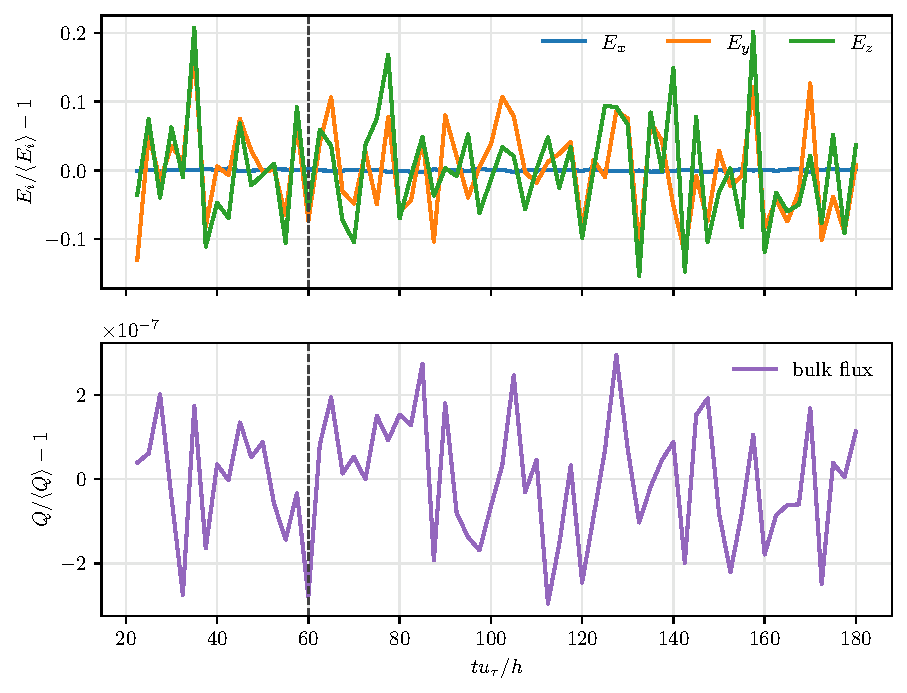
\includegraphics[width=0.86\linewidth]{figures/mkm_production_sampling_diagnostics.pdf}
  \caption{Sampling-stage scalar diagnostics. Upper panel: kinetic-energy
  components \(E_x\), \(E_y\), and \(E_z\), plotted as relative deviations
  from their own sampling means. Lower panel: bulk flux \(Q\), plotted as a
  relative deviation from its sampling mean. The abscissa is \(t u_{\tau}/h\),
  and the dashed line marks the retained-window start
  \(t u_{\tau}/h=60\).}
  \label{fig:diagnostics}
\end{figure}

\subsection{Instantaneous and mean velocity contours}

Figures~\ref{fig:instantaneous_contours} and \ref{fig:mean_contours} separate
the instantaneous and mean streamwise-velocity contours. This layout preserves
the equal physical aspect ratio of each slice and keeps each colorbar aligned
with the height of its corresponding contour. The instantaneous
\((x/h,z/h)\) slice fixes a spanwise index and displays \(u_x/u_{\tau}\), while
the instantaneous \((y/h,z/h)\) slice fixes a streamwise index and displays the
same nondimensional velocity. The mean contours are horizontally homogeneous
by construction, since the estimator in Eq.~\eqref{eq:mean_profile} averages
over both periodic directions.

\begin{figure}[H]
  \centering
  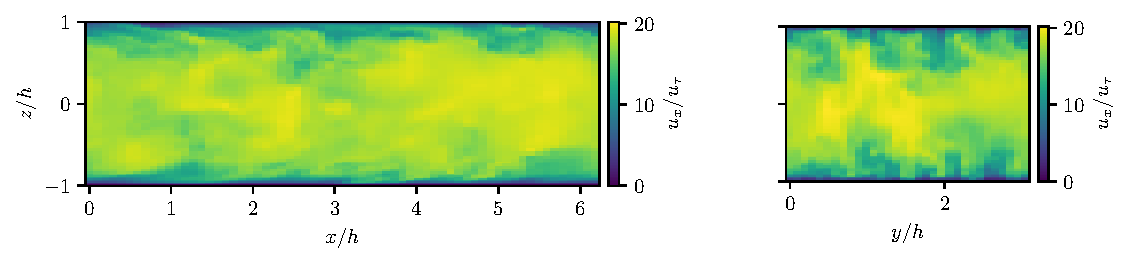
\includegraphics[width=0.95\linewidth]{figures/mkm_production_instantaneous_contours.pdf}
  \caption{Instantaneous streamwise velocity \(u_x/u_{\tau}\) at
  \(t u_{\tau}/h=180\). Left panel: streamwise-normal \((x/h,z/h)\) slice at
  \(y/h=0\). Right panel: spanwise-normal \((y/h,z/h)\) slice at \(x/h=0\).}
  \label{fig:instantaneous_contours}
\end{figure}

\begin{figure}[H]
  \centering
  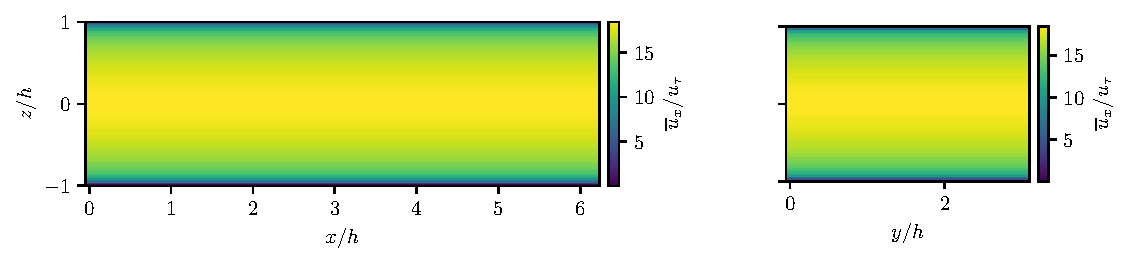
\includegraphics[width=0.95\linewidth]{figures/mkm_production_mean_contours.pdf}
  \caption{Accepted mean streamwise velocity \(\overline{u}_x/u_{\tau}\) over
  the \(60\le t u_{\tau}/h\le180\) target window. Left panel: the wall-normal
  mean replicated along \(x/h\). Right panel: the same mean replicated along
  \(y/h\).}
  \label{fig:mean_contours}
\end{figure}

\subsection{Mean and Reynolds-stress profiles}

Figure~\ref{fig:mean_profile_result} shows the accepted mean velocity profile.
The streamwise component has the expected channel-flow profile, while the
spanwise and wall-normal mean components remain small compared with
\(\overline{u}_x\). The profile is plotted as \(\overline{u}_i/u_{\tau}\)
against \(z/h\). Figure~\ref{fig:reynolds_profile_result} shows the six
independent components of the Reynolds-stress tensor profile
\(R_{\alpha\beta}/u_{\tau}^2\) against \(z/h\). The off-diagonal component
\(R_{xz}\) carries the dominant shear-stress structure; the other off-diagonal
components are small on this scale.

\begin{figure}[H]
  \centering
  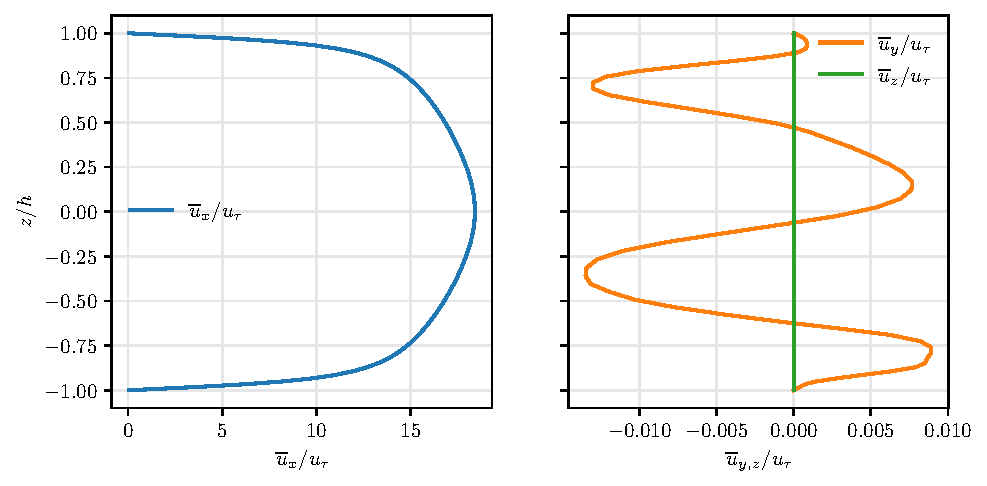
\includegraphics[width=0.95\linewidth]{figures/mkm_production_mean_velocity_profile.pdf}
  \caption{Accepted mean velocity profile computed from the
  \(60\le t u_{\tau}/h\le180\) target window. Left panel: streamwise mean
  \(\overline{u}_x/u_{\tau}\). Right panel: secondary means
  \(\overline{u}_y/u_{\tau}\) and \(\overline{u}_z/u_{\tau}\).}
  \label{fig:mean_profile_result}
\end{figure}

\begin{figure}[H]
  \centering
  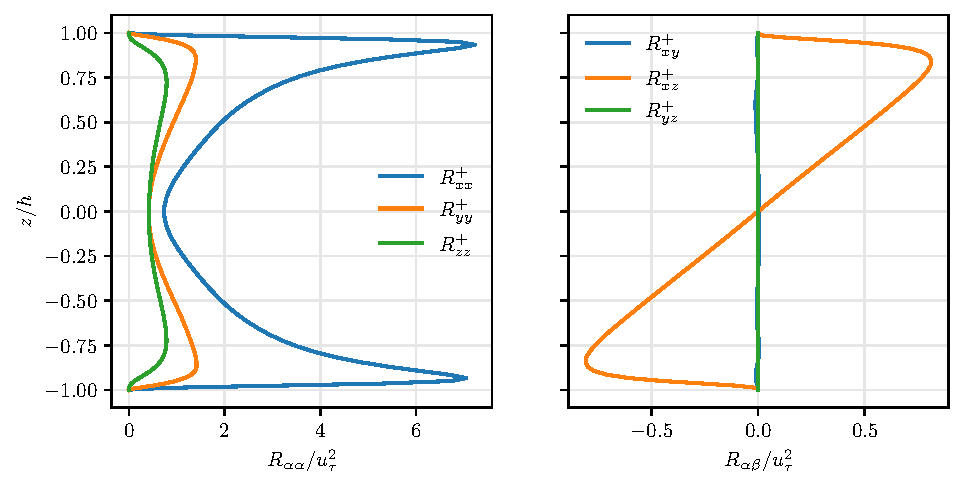
\includegraphics[width=0.95\linewidth]{figures/mkm_production_reynolds_stress_profiles.pdf}
  \caption{Accepted Reynolds-stress tensor profile computed from the
  \(60\le t u_{\tau}/h\le180\) target window. Left panel: diagonal components
  \(R_{xx}/u_{\tau}^2\), \(R_{yy}/u_{\tau}^2\), and \(R_{zz}/u_{\tau}^2\).
  Right panel: off-diagonal components \(R_{xy}/u_{\tau}^2\),
  \(R_{xz}/u_{\tau}^2\), and \(R_{yz}/u_{\tau}^2\).}
  \label{fig:reynolds_profile_result}
\end{figure}

\subsection{Plane-averaged temporal auto-covariances and auto-spectra}
\label{subsec:temporal_autocovariance_autospectrum}

The covariance and spectral quantities in the preceding sections are equal-time
statistics. For a reproduction run with explicit temporal dynamics, it is also
useful to record height-resolved temporal statistics in physical space. The
accepted equal-time target uses the \(60\le t u_{\tau}/h\le180\) production
window described above. The temporal figures in this subsection instead use a
separate dense continuation restarted from the final \(t u_{\tau}/h=180\)
checkpoint and sampled every 20 DNS steps. This keeps the equal-time target
unchanged while improving the temporal lag spacing and frequency range.

Let the dense sample times, measured from the first dense snapshot, be
\[
  t_n=n\Delta t_s,\qquad n=0,\ldots,N_s-1,
\]
where the absolute dense-window range is
\[
  180.01 \le t_{\mathrm{abs}}u_{\tau}/h \le 300,
\]
\(N_s=12000\), and
\[
  \Delta t_s u_{\tau}/h = 0.01.
\]
The sample spacing \(\Delta t_s\) is the snapshot spacing, not the DNS solver
step. For a velocity component \(i\in\{x,y,z\}\), define
\[
  u'_i(x_j,y_\ell,z_m,t_n)
  =
  u_i(x_j,y_\ell,z_m,t_n)-\overline{u}^{\,\mathrm{dense}}_i(z_m),
\]
where \(\overline{u}^{\,\mathrm{dense}}_i(z_m)\) is recomputed from the dense
continuation samples. This dense temporal mean is used only for the temporal
diagnostics; the target mean profile in Eq.~\eqref{eq:mean_profile} remains the
accepted \(60\le t u_{\tau}/h\le180\) estimator.
For an integer lag \(s\ge0\), let
\[
  \tau_s=s\Delta t_s.
\]
The plane-averaged positive-lag auto-covariance at height \(z_m\) is estimated
by
\begin{equation}
  R_{ii}(\tau_s;z_m)
  =
  \frac{1}{(N_s-s)N_xN_y}
  \sum_{n=0}^{N_s-s-1}
  \sum_{j=0}^{N_x-1}
  \sum_{\ell=0}^{N_y-1}
  u'_i(x_j,y_\ell,z_m,t_{n+s})
  u'_i(x_j,y_\ell,z_m,t_n).
  \label{eq:plane_autocovariance_estimator}
\end{equation}
This is the direct finite-sample approximation of
\[
  \mathbb{E}\left[
  u_i'(t+\tau,x,y,z_m)u_i'(t,x,y,z_m)
  \right],
\]
with the expectation replaced by an average over admissible time origins and
over the statistically homogeneous \(x\)--\(y\) plane. The factor
\((N_s-s)^{-1}\) appears because only \(N_s-s\) pairs are available at lag
\(s\), and the dimensionless correlation is
\begin{equation}
  \rho_{ii}(\tau_s;z_m)
  =
  \frac{R_{ii}(\tau_s;z_m)}{R_{ii}(0;z_m)}.
  \label{eq:plane_autocorrelation_definition}
\end{equation}
Equation~\eqref{eq:plane_autocorrelation_definition} is dimensionless and is
plotted against \(\tau_su_{\tau}/h\).

The corresponding auto-spectrum is computed by a temporal Fourier transform
at each fixed \((x_j,y_\ell,z_m)\), followed by the same horizontal-plane
average. The angular frequencies associated with the \(N_s\)-point temporal
FFT are
\begin{equation}
  \omega_r
  =
  2\pi\,\mathrm{fftfreq}(N_s,\Delta t_s)_r .
  \label{eq:temporal_omega_grid}
\end{equation}
For the dense continuation,
\[
  \Delta\omega^*=\frac{2\pi}{N_s\Delta t_s}\frac{h}{u_\tau}
  = 0.0523598775599,
\]
and the plotted positive branch extends to
\[
  \omega^*_{\max}=314.106905482,
\]
with Nyquist magnitude \(\pi/\Delta t_s\simeq314.159265359\).
Let \(w_n\) be an optional temporal window and define the corresponding
frequency-indexed Fourier coefficient by
\begin{equation}
  \widetilde{u}_{i}(x_j,y_\ell,z_m;\omega_r)
  =
  \sum_{n=0}^{N_s-1}
  w_n u'_i(x_j,y_\ell,z_m,t_n)
  \exp\left(-2\pi\ii\frac{rn}{N_s}\right),
  \qquad r=0,\ldots,N_s-1.
  \label{eq:temporal_dft_definition}
\end{equation}
With the unnormalized discrete Fourier transform in
Eq.~\eqref{eq:temporal_dft_definition}, the two-sided plane-averaged
periodogram is
\begin{equation}
  S_{ii}(\omega_r;z_m)
  =
  \frac{\Delta t_s}{N_xN_y\sum_{n=0}^{N_s-1}w_n^2}
  \sum_{j=0}^{N_x-1}
  \sum_{\ell=0}^{N_y-1}
  \left|
  \widetilde{u}_{i}(x_j,y_\ell,z_m;\omega_r)
  \right|^2 .
  \label{eq:plane_autospectrum_estimator}
\end{equation}
The dense auto-spectrum figure uses a Hann window. The formula records the
normalization for a general window because smoothing is useful for this finite
temporal record.

The normalization in Eq.~\eqref{eq:plane_autospectrum_estimator} is chosen to
be consistent with the two-sided angular-frequency convention. To see this,
first consider \(w_n=1\), for which \(\sum_n w_n^2=N_s\). The angular-frequency
spacing is
\[
  \Delta\omega=\frac{2\pi}{N_s\Delta t_s}.
\]
Parseval's identity for the unnormalized transform gives
\[
  \sum_{r=0}^{N_s-1}
  \left|\widetilde{u}_{i}(x_j,y_\ell,z_m;\omega_r)\right|^2
  =
  N_s
  \sum_{n=0}^{N_s-1}
  \left|u'_i(x_j,y_\ell,z_m,t_n)\right|^2 .
\]
Therefore,
\begin{align}
  \frac{1}{2\pi}
  \sum_{r=0}^{N_s-1}
  S_{ii}(\omega_r;z_m)\Delta\omega
  &=
  \frac{1}{N_s\Delta t_s}
  \sum_{r=0}^{N_s-1}
  \frac{\Delta t_s}{N_sN_xN_y}
  \sum_{j,\ell}
  \left|\widetilde{u}_{i}(x_j,y_\ell,z_m;\omega_r)\right|^2
  \nonumber\\
  &=
  \frac{1}{N_s^2N_xN_y}
  \sum_{j,\ell}
  N_s\sum_{n=0}^{N_s-1}
  \left|u'_i(x_j,y_\ell,z_m,t_n)\right|^2
  \nonumber\\
  &=
  \frac{1}{N_sN_xN_y}
  \sum_{n,j,\ell}
  \left|u'_i(x_j,y_\ell,z_m,t_n)\right|^2
  =
  R_{ii}(0;z_m).
  \label{eq:periodogram_parseval_check}
\end{align}
Thus, for a rectangular window, the discrete sum of the two-sided periodogram
recovers the zero-lag plane-averaged variance. For a nontrivial window such as
the Hann window used below, the same calculation recovers the corresponding
window-energy-weighted zero-lag estimate. For
Figure~\ref{fig:velocity_autospectrum_result}, the dimensional spectrum is
normalized by its own discrete two-sided spectral area and then
nondimensionalized as
\[
  S_{ii}^*(\omega_r;z_m)
  =
  \frac{S_{ii}(\omega_r;z_m)u_{\tau}}
       {hR^{S}_{ii}(0;z_m)},
  \qquad
  \omega_r^*=\frac{\omega_r h}{u_{\tau}}.
\]
Here \(R^{S}_{ii}(0;z_m)\) denotes the zero-lag variance implied by the
discrete spectral area. This scaling is dimensionless because
\([S_{ii}/R^{S}_{ii}(0;z_m)]=[t]\), and it gives the normalized two-sided area
identity
\[
  \frac{1}{2\pi}\sum_{r=0}^{N_s-1}
  S_{ii}^*(\omega_r;z_m)\Delta\omega^*
  = 1,
  \qquad
  \Delta\omega^*=\Delta\omega\,h/u_{\tau}.
\]

\begin{figure}[H]
  \centering
  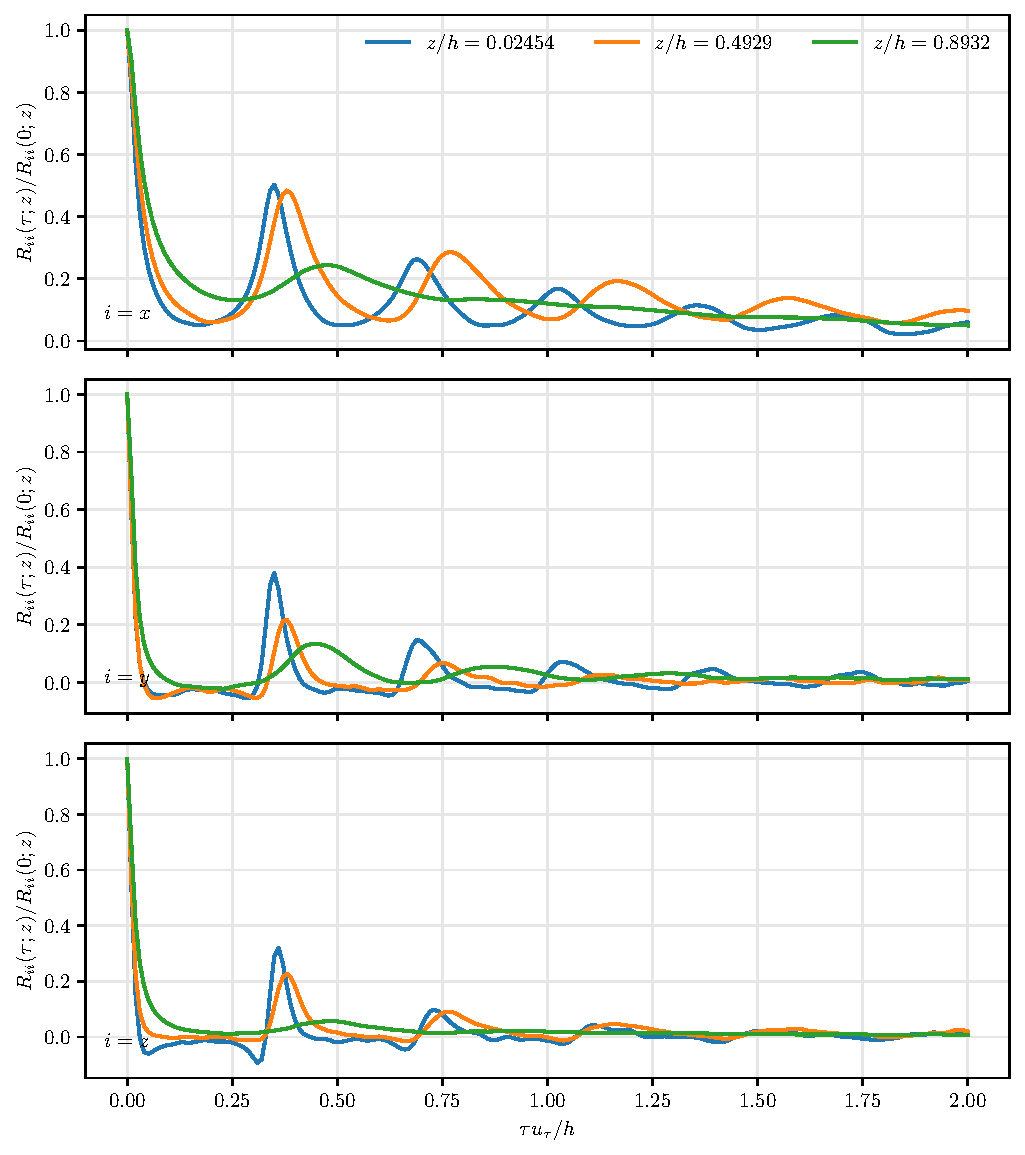
\includegraphics[width=0.95\linewidth]{figures/mkm_velocity_autocovariance_selected_z.pdf}
  \caption{Plane-averaged temporal auto-correlation
  \(R_{ii}(\tau;z)/R_{ii}(0;z)\) from the dense temporal continuation. The
  three panels correspond to \(i=x\), \(i=y\), and \(i=z\), as indicated inside
  each panel. Curves show one nonsymmetric half-channel set of wall-normal
  levels, namely the nearest saved Chebyshev-Gauss levels to
  \(z/h=0,0.5,0.9\). The abscissa is the nondimensional lag
  \(\tau u_{\tau}/h\), sampled at increments of \(0.01\).}
  \label{fig:velocity_autocovariance_result}
\end{figure}

\begin{figure}[H]
  \centering
  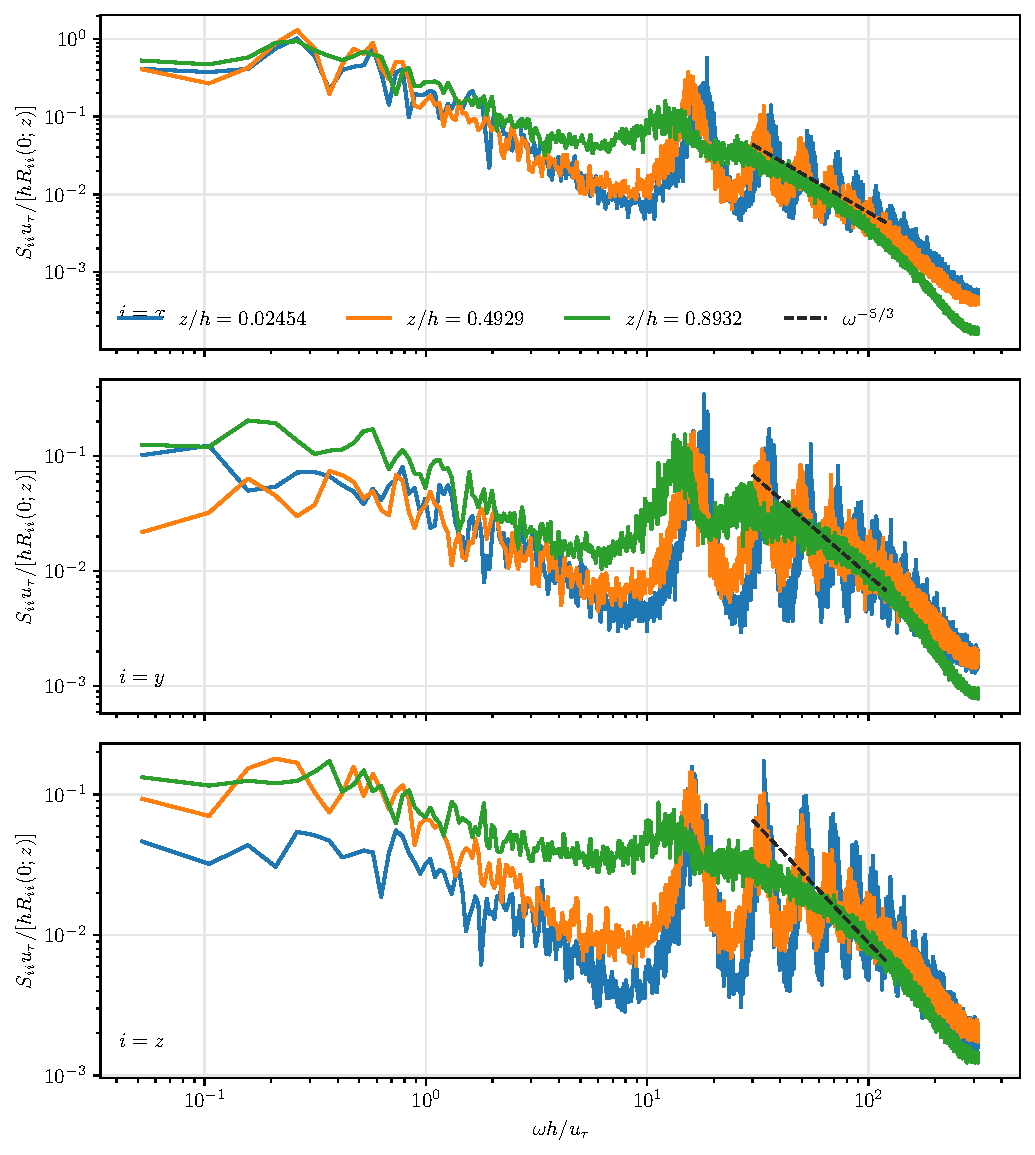
\includegraphics[width=0.95\linewidth]{figures/mkm_velocity_autospectrum_selected_z_loglog.pdf}
  \caption{Plane-averaged temporal auto-spectrum computed from the dense
  temporal continuation using a Hann window. The plotted quantity is the
  variance-normalized spectrum \(S_{ii}(\omega;z)u_{\tau}/[hR^S_{ii}(0;z)]\)
  against
  \(\omega h/u_{\tau}\), using the positive branch of the two-sided
  angular-frequency periodogram. With this normalization, the two-sided
  spectral area equals unity for each component and wall-normal level. The
  three panels correspond to \(i=x\), \(i=y\), and \(i=z\), as indicated inside
  each panel. Curves show one nonsymmetric half-channel set of wall-normal
  levels, namely the nearest saved Chebyshev-Gauss levels to
  \(z/h=0,0.5,0.9\). The dashed line gives a \(\omega^{-5/3}\) reference
  slope.}
  \label{fig:velocity_autospectrum_result}
\end{figure}

The auto-correlation in Figure~\ref{fig:velocity_autocovariance_result} shows
a clear separation between the streamwise component and the two secondary
components. The streamwise fluctuations retain a positive correlation over the
entire plotted range \(0\le\tau u_{\tau}/h\le2\), with the outer half-channel
level remaining more correlated than the near-center level after the first few
tenths of a turnover time. This behavior is consistent with long streamwise
structures in a channel flow and with the dominance of \(R_{xx}\) in
Figure~\ref{fig:reynolds_profile_result}. In contrast, the spanwise and
wall-normal components decorrelate rapidly: after
\(\tau u_{\tau}/h\approx0.1\)--\(0.2\), now resolved by roughly 10--20 dense
sample intervals, their correlations fluctuate around zero with only
finite-sample oscillations. The one-sided wall-normal selection is used only to
avoid duplicating approximately symmetric information. The dense continuation
starts from the accepted production final state and is used here for temporal
resolution, not as a replacement for the equal-time target.

The log-log spectra in Figure~\ref{fig:velocity_autospectrum_result} give the
same information in the frequency domain after removing the trivial variance
amplitude at each height. The streamwise spectra retain relatively more
low-frequency content than the spanwise and wall-normal spectra, particularly
near the outer half-channel level. The spanwise and wall-normal spectra have
shorter-correlation signatures, with comparatively flatter high-frequency
floors once normalized by \(R^S_{ii}(0;z)\). Relative to the original
\(\Delta t_s u_\tau/h=0.1\) production snapshots, the dense continuation extends
the plotted positive branch by approximately one decade, to
\(\omega h/u_\tau\simeq314\), and refines the lag spacing by the same factor.
The dashed \(\omega^{-5/3}\) segment is included only as a log-log slope
reference over \(\omega h/u_\tau=30\)--\(120\); the finite temporal record and
single-record periodogram should not be interpreted as an inertial-range fit.
By construction, the variance-normalized two-sided spectral area is one for
every plotted component and wall-normal level.

\subsection{Target layout and constraint audit}

The accepted target contains the following key shapes:
\[
\begin{array}{ll}
\texttt{mean\_profile}: & (64,3),\\
\texttt{reynolds\_stress\_profile}: & (64,3,3),\\
\texttt{modal/u\_hat}: & (1201,64,32,192),\\
\texttt{modal/B0\_DNS}: & (64,32,192,192),\\
\texttt{lag\_covariance/lag\_0}: & (64,32,192,192),\\
\texttt{lag\_covariance/lag\_1}: & (64,32,192,192).
\end{array}
\]
The target file size is
\[
  11181644712\ \text{bytes}.
\]

The Chebyshev-quadrature constraint file is
\[
  \texttt{MKM\_constraints\_N64\_64\_32\_cheb\_quadrature\_spectral.h5}.
\]
Its rank audit gives one rank-68 mode and 2047 rank-70 modes:
\[
  \#\{ \operatorname{rank}=68\}=1,\qquad
  \#\{ \operatorname{rank}=70\}=2047.
\]
The final audit confirms that the target grid matches both the saved velocity
grid and the saved Chebyshev-quadrature constraint grid:
\[
  \texttt{z\_grid\_match\_velocity}=\texttt{true},\qquad
  \texttt{z\_grid\_match\_constraint}=\texttt{true}.
\]
The global residual of the sampled modal covariance under the saved constraint
was
\[
  \frac{\|\Gtilde\widehat{\bfq}\|}{\|\widehat{\bfq}\|}
  \approx 5.32\times 10^{-14},
\]
with divergence and boundary contributions
\[
  5.32\times 10^{-14}
  \quad\text{and}\quad
  4.16\times 10^{-16},
\]
respectively. These values are near machine precision for the present
postprocessing and confirm consistency between the accepted target covariance
and the solver-native Chebyshev/quadrature constraint.

\section{Admissible projection of the sampled covariance}
\label{sec:projected_covariance}

The preceding audit checks the sampled modal coefficients directly. In this
section we also construct the covariance that would be obtained by explicitly
projecting the sampled equal-time covariance onto the discrete admissible
subspace. This is the covariance denoted by
\(\Badm(\kappa_p,\lambda_q)\). The calculation provides an independent
end-to-end check that the stored covariance, the saved constraint recipe, and
the sampled Reynolds-stress profiles are mutually consistent.

\subsection{Notation for one horizontal mode}

Fix one horizontal Fourier mode \((\kappa_p,\lambda_q)\), and let
\[
  d = 3N_z.
\]
The stored equal-time DNS covariance for this mode is
\[
  \Bzero^{pq}
  =
  \frac{1}{N_s}
  \sum_{n=0}^{N_s-1}
  \widehat{\bfq}_{pq}(t_n)
  \widehat{\bfq}_{pq}(t_n)^*
  \in\mathbb{C}^{d\times d},
  \label{eq:project_b0_definition}
\]
with the same level-major component ordering as in
Eq.~\eqref{eq:modal_vector}. The row-orthonormal constraint matrix for the
same mode is
\begin{equation}
  \Gtilde_{pq}\in\mathbb{C}^{r_{pq}\times d},
  \qquad
  \Gtilde_{pq}\Gtilde_{pq}^*=I_{r_{pq}},
  \label{eq:project_gtilde_rows}
\end{equation}
where \(r_{pq}\) is the numerical rank of \(\Graw(\kappa_p,\lambda_q)\).
The admissible modal subspace is
\[
  \mathcal{A}_{pq}
  =
  \left\{v\in\mathbb{C}^{d}:\Gtilde_{pq}v=0\right\}.
  \label{eq:admissible_subspace}
\]

\subsection{Derivation of the orthogonal projector}

Because the rows of \(\Gtilde_{pq}\) are orthonormal, the matrix
\[
  \Gtilde_{pq}^*\Gtilde_{pq}
\]
is the orthogonal projector onto the row space of \(\Gtilde_{pq}\). Indeed,
for any vector \(v\in\mathbb{C}^d\), the row-space component is obtained by
first taking row coordinates \(\Gtilde_{pq}v\), and then mapping those
coordinates back into the physical modal-vector space with \(\Gtilde_{pq}^*\).
The complementary projector is therefore
\begin{equation}
  \Pmat_{pq}
  =
  I_d-\Gtilde_{pq}^*\Gtilde_{pq}.
  \label{eq:admissible_projector}
\end{equation}
This matrix is Hermitian, since
\[
  \Pmat_{pq}^*
  =
  I_d-\Gtilde_{pq}^*\Gtilde_{pq}
  =
  \Pmat_{pq}.
\]
It is also idempotent:
\begin{align}
  \Pmat_{pq}^2
  &=
  \left(I_d-\Gtilde_{pq}^*\Gtilde_{pq}\right)
  \left(I_d-\Gtilde_{pq}^*\Gtilde_{pq}\right) \nonumber\\
  &=
  I_d-2\Gtilde_{pq}^*\Gtilde_{pq}
  +\Gtilde_{pq}^*
   \left(\Gtilde_{pq}\Gtilde_{pq}^*\right)
   \Gtilde_{pq} \nonumber\\
  &=
  I_d-\Gtilde_{pq}^*\Gtilde_{pq}
  =
  \Pmat_{pq},
  \label{eq:projector_idempotent}
\end{align}
where Eq.~\eqref{eq:project_gtilde_rows} was used in the penultimate line.
Finally,
\[
  \Gtilde_{pq}\Pmat_{pq}
  =
  \Gtilde_{pq}
  -
  \left(\Gtilde_{pq}\Gtilde_{pq}^*\right)\Gtilde_{pq}
  =
  0,
\]
so the range of \(\Pmat_{pq}\) is contained in \(\mathcal{A}_{pq}\). If
\(v\in\mathcal{A}_{pq}\), then \(\Gtilde_{pq}v=0\), and
\(\Pmat_{pq}v=v\). Thus Eq.~\eqref{eq:admissible_projector} is exactly the
orthogonal projector onto the admissible subspace.

\subsection{Projected covariance}

Let \(\widehat{\bfq}_{pq}\) denote a zero-mean random modal vector with
covariance \(\Bzero^{pq}\). Its admissible projection is
\[
  \widehat{\bfq}_{pq}^{\,\mathrm{adm}}
  =
  \Pmat_{pq}\widehat{\bfq}_{pq}.
\]
Taking the covariance of this projected vector gives
\begin{align}
  \Badm^{pq}
  &=
  \mathbb{E}\left[
    \widehat{\bfq}_{pq}^{\,\mathrm{adm}}
    \left(\widehat{\bfq}_{pq}^{\,\mathrm{adm}}\right)^*
  \right] \nonumber\\
  &=
  \mathbb{E}\left[
    \Pmat_{pq}\widehat{\bfq}_{pq}
    \widehat{\bfq}_{pq}^*
    \Pmat_{pq}^*
  \right] \nonumber\\
  &=
  \Pmat_{pq}
  \mathbb{E}\left[
    \widehat{\bfq}_{pq}\widehat{\bfq}_{pq}^*
  \right]
  \Pmat_{pq}^* \nonumber\\
  &=
  \Pmat_{pq}\Bzero^{pq}\Pmat_{pq},
  \label{eq:projected_covariance_definition}
\end{align}
because \(\Pmat_{pq}^*=\Pmat_{pq}\). Equation
\eqref{eq:projected_covariance_definition} is the covariance used by a
generator that enforces the discrete incompressibility and no-slip constraints
exactly at the modal-covariance level.

\subsection{Exact equality for constrained DNS samples}
\label{subsec:exact_b0_badm_equality}

The near-zero difference between \(\Bzero^{pq}\) and \(\Badm^{pq}\) is not an
independent empirical coincidence. It follows algebraically from using the
same discrete constraint in the DNS target and in the projection. Suppose that
each sampled modal coefficient satisfies the saved constraint exactly,
\begin{equation}
  \Gtilde_{pq}\widehat{\bfq}_{pq}(t_n)=0,
  \qquad n=0,\ldots,N_s-1.
  \label{eq:sample_coefficients_exactly_constrained}
\end{equation}
Then every sample belongs to the admissible subspace
\(\mathcal{A}_{pq}\). Since \(\Pmat_{pq}\) is the identity on this subspace,
\begin{equation}
  \Pmat_{pq}\widehat{\bfq}_{pq}(t_n)
  =
  \widehat{\bfq}_{pq}(t_n).
  \label{eq:projector_identity_on_samples}
\end{equation}
Applying Eq.~\eqref{eq:projector_identity_on_samples} to the finite-sample
covariance estimator gives
\begin{align}
  \Pmat_{pq}\Bzero^{pq}\Pmat_{pq}
  &=
  \Pmat_{pq}
  \left[
  \frac{1}{N_s}
  \sum_{n=0}^{N_s-1}
  \widehat{\bfq}_{pq}(t_n)
  \widehat{\bfq}_{pq}(t_n)^*
  \right]
  \Pmat_{pq} \nonumber\\
  &=
  \frac{1}{N_s}
  \sum_{n=0}^{N_s-1}
  \left(\Pmat_{pq}\widehat{\bfq}_{pq}(t_n)\right)
  \left(\Pmat_{pq}\widehat{\bfq}_{pq}(t_n)\right)^* \nonumber\\
  &=
  \frac{1}{N_s}
  \sum_{n=0}^{N_s-1}
  \widehat{\bfq}_{pq}(t_n)
  \widehat{\bfq}_{pq}(t_n)^*
  =
  \Bzero^{pq}.
  \label{eq:b0_equals_projected_b0_samplewise}
\end{align}
Combining Eqs.~\eqref{eq:projected_covariance_definition} and
\eqref{eq:b0_equals_projected_b0_samplewise} yields the exact identity
\begin{equation}
  \Badm^{pq}=\Bzero^{pq}
  \label{eq:badm_equals_b0_exact}
\end{equation}
for every horizontal mode whose sampled coefficients satisfy
Eq.~\eqref{eq:sample_coefficients_exactly_constrained}.

The same result can be written as a covariance-range statement. From
Eq.~\eqref{eq:sample_coefficients_exactly_constrained},
\begin{align}
  \Gtilde_{pq}\Bzero^{pq}
  &=
  \frac{1}{N_s}
  \sum_{n=0}^{N_s-1}
  \left(\Gtilde_{pq}\widehat{\bfq}_{pq}(t_n)\right)
  \widehat{\bfq}_{pq}(t_n)^*
  =
  0, \label{eq:gb0_zero}\\
  \Bzero^{pq}\Gtilde_{pq}^*
  &=
  \left(\Gtilde_{pq}\Bzero^{pq}\right)^*
  =
  0. \label{eq:b0gstar_zero}
\end{align}
Substituting Eqs.~\eqref{eq:gb0_zero} and \eqref{eq:b0gstar_zero} into the
direct expansion of \(\Pmat_{pq}\Bzero^{pq}\Pmat_{pq}\) gives
\begin{align}
  \Pmat_{pq}\Bzero^{pq}\Pmat_{pq}
  &=
  \Bzero^{pq}
  -
  \Gtilde_{pq}^*\Gtilde_{pq}\Bzero^{pq}
  -
  \Bzero^{pq}\Gtilde_{pq}^*\Gtilde_{pq}
  +
  \Gtilde_{pq}^*\Gtilde_{pq}
  \Bzero^{pq}
  \Gtilde_{pq}^*\Gtilde_{pq} \nonumber\\
  &=
  \Bzero^{pq}.
  \label{eq:range_proof_b0_projection}
\end{align}
Hence the projection cannot change a covariance assembled from exactly
constrained samples. Any nonzero \(\|\Badm^{pq}-\Bzero^{pq}\|\) in the
production calculation is therefore a finite-precision diagnostic: it measures
floating-point roundoff, SVD compression and reconstruction tolerances, and
HDF5 read/write arithmetic, not a physical or statistical modification of the
target covariance.

The implementation evaluates Eq.~\eqref{eq:projected_covariance_definition}
from the stored data. If a dense \(\Gtilde_{pq}\) is present in the constraint
file, it is read directly. The production constraint file stores seven
representative compressed matrices by default; for the remaining modes, the
postprocessor reconstructs \(\Gtilde_{pq}\) from the saved arrays
\(\Dz\), \(\Bbdry\), \(\Ex\), \(\Ey\), \(\Ez\), \(\kappa_p\), and
\(\lambda_q\) by applying the same SVD compression derived in
Section~\ref{sec:constraint}. Thus all ingredients are taken from the target
and constraint HDF5 files. The numerical formula used in the script is the
expanded form
\begin{align}
  \Badm^{pq}
  &=
  \Bzero^{pq}
  -
  \Gtilde_{pq}^*\Gtilde_{pq}\Bzero^{pq}
  -
  \Bzero^{pq}\Gtilde_{pq}^*\Gtilde_{pq} \nonumber\\
  &\quad
  +
  \Gtilde_{pq}^*\Gtilde_{pq}
  \Bzero^{pq}
  \Gtilde_{pq}^*\Gtilde_{pq},
  \label{eq:projected_covariance_expanded}
\end{align}
followed by explicit Hermitian symmetrization at roundoff level.

\subsection{Reynolds stresses reproduced from a modal covariance}

The sampled Reynolds-stress profile can also be reconstructed from any modal
covariance \(C^{pq}\) with the same Fourier normalization as the target file.
Let \(s(x)=0\), \(s(y)=1\), and \(s(z)=2\), and define the level-major index
\[
  \ell(m,\alpha)=3m+s(\alpha).
\]
The inverse horizontal Fourier representation of the fluctuation field is
\[
  u'_\alpha(x_j,y_\ell,z_m)
  =
  \sum_{p=0}^{N_x-1}
  \sum_{q=0}^{N_y-1}
  \widehat{u}_\alpha(z_m;\kappa_p,\lambda_q)
  \exp\left[\ii(\kappa_p x_j+\lambda_q y_\ell)\right],
  \label{eq:inverse_fft_for_reynolds}
\]
because the forward transform in Eq.~\eqref{eq:fft_coeff} already contains the
factor \(1/(N_xN_y)\). Multiplying two components and averaging over the
horizontal grid gives
\begin{align}
  \left\langle
  u'_\alpha u'_\beta
  \right\rangle_{xy}
  &=
  \sum_{p,q}
  \sum_{p',q'}
  \widehat{u}_\alpha(z_m;\kappa_p,\lambda_q)
  \widehat{u}_\beta(z_m;\kappa_{p'},\lambda_{q'})^*
  \left\langle
    e^{\ii[(\kappa_p-\kappa_{p'})x
          +(\lambda_q-\lambda_{q'})y]}
  \right\rangle_{xy}.
  \label{eq:reynolds_parseval_start}
\end{align}
The discrete Fourier modes are orthogonal on the sampled periodic grid, so
\[
  \left\langle
    e^{\ii[(\kappa_p-\kappa_{p'})x
          +(\lambda_q-\lambda_{q'})y]}
  \right\rangle_{xy}
  =
  \delta_{pp'}\delta_{qq'}.
\]
Therefore only equal horizontal modes survive, and the Reynolds-stress profile
implied by \(C^{pq}\) is
\begin{equation}
  R_{\alpha\beta}^{C}(z_m)
  =
  \sum_{p=0}^{N_x-1}
  \sum_{q=0}^{N_y-1}
  C^{pq}_{\ell(m,\alpha),\ell(m,\beta)}.
  \label{eq:reynolds_from_modal_covariance}
\end{equation}
No additional \(N_xN_y\) factor appears in Eq.~\eqref{eq:reynolds_from_modal_covariance};
it has already been fixed by the forward and inverse transform convention.
In the comparison below, Eq.~\eqref{eq:reynolds_from_modal_covariance} is
evaluated for both \(C^{pq}=\Bzero^{pq}\) and
\(C^{pq}=\Badm^{pq}\).

\subsection{Production computation and comparison}

The projected covariance was computed with
\[
  \texttt{scripts/mkm\_dns\_target/project\_mkm\_dns\_covariance.py}.
\]
For the production data set, the script wrote
\[
  \texttt{MKM\_production\_64\_64\_32\_projected\_covariance\_t60\_t180.h5},
\]
which contains \(\Badm^{pq}\), the Reynolds profiles implied by
\(\Bzero\) and \(\Badm\), and modewise projection diagnostics. The run
processed all \(64\times32=2048\) horizontal modes. Seven \(\Gtilde_{pq}\)
matrices were read directly from saved representative-mode groups, and the
remaining 2041 were reconstructed from the saved constraint operators.

\begin{table}[H]
  \centering
  \caption{Projection and Reynolds-stress consistency diagnostics for the
  accepted \(60\le t u_{\tau}/h\le180\) production target. Norms are Frobenius
  norms unless otherwise stated.}
  \label{tab:projected_covariance_diagnostics}
  \begin{tabular}{lr}
    \toprule
    Diagnostic & Value \\
    \midrule
    Global \(\|\Badm-\Bzero\|/\|\Bzero\|\) & \(1.1046\times10^{-15}\) \\
    Maximum modewise \(\|\Badm^{pq}-\Bzero^{pq}\|/\|\Bzero^{pq}\|\) & \(5.6548\times10^{-15}\) \\
    Relative trace change \((\mathrm{tr}\,\Badm-\mathrm{tr}\,\Bzero)/\mathrm{tr}\,\Bzero\) & \(0.0\) \\
    Total \(\mathrm{tr}\,\Bzero\) & \(260.3681545\) \\
    Maximum projected constraint residual & \(8.8989\times10^{-17}\) \\
    \(\|R^{\Bzero}-R^{\mathrm{sample}}\|/\|R^{\mathrm{sample}}\|\) & \(2.9426\times10^{-15}\) \\
    \(\|R^{\Badm}-R^{\mathrm{sample}}\|/\|R^{\mathrm{sample}}\|\) & \(2.9326\times10^{-15}\) \\
    \(\|R^{\Badm}-R^{\Bzero}\|/\|R^{\Bzero}\|\) & \(2.0371\times10^{-16}\) \\
    \(\max |R^{\Badm}-R^{\mathrm{sample}}|\) & \(3.8192\times10^{-14}\) \\
    \bottomrule
  \end{tabular}
\end{table}

The values in Table~\ref{tab:projected_covariance_diagnostics} are therefore
best interpreted as a finite-precision verification of
Eq.~\eqref{eq:badm_equals_b0_exact}. The exact-arithmetic prediction is that
the explicit projection leaves the production equal-time covariance unchanged.
The observed \(10^{-15}\)-level changes are consistent with the direct
modal-coefficient audit in Section~\ref{sec:production_results}: the sampled
velocity coefficients already satisfy the saved Chebyshev/quadrature
divergence and no-slip constraints to near machine precision.

\begin{figure}[H]
  \centering
  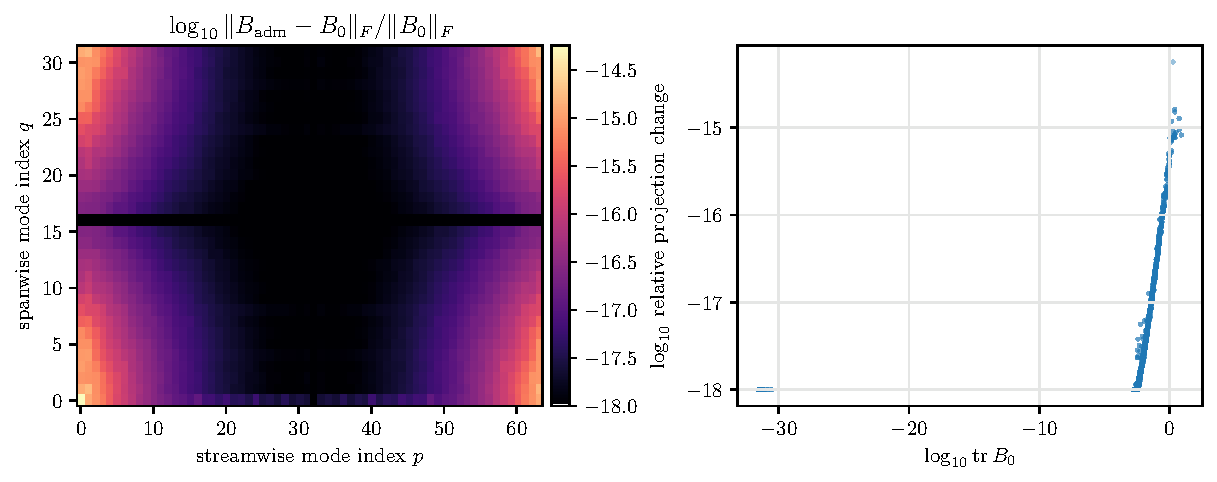
\includegraphics[width=0.95\linewidth]{figures/mkm_projected_covariance_mode_errors.pdf}
  \caption{Modewise finite-precision effect of the admissible covariance
  projection. Left:
  relative Frobenius-norm change
  \(\|\Badm^{pq}-\Bzero^{pq}\|_F/\|\Bzero^{pq}\|_F\). Right: the same relative
  projection change plotted against modal covariance energy
  \(\mathrm{tr}\,\Bzero^{pq}\).}
  \label{fig:projected_covariance_mode_errors}
\end{figure}

\begin{figure}[H]
  \centering
  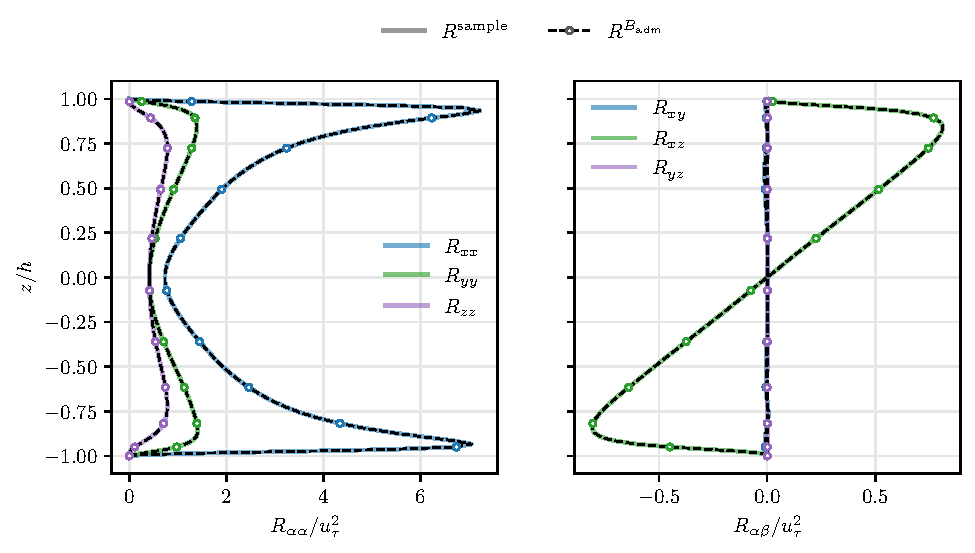
\includegraphics[width=0.95\linewidth]{figures/mkm_projected_reynolds_stress_profiles.pdf}
  \caption{Reynolds-stress profiles from the sampled physical-space estimator
  and from the projected modal covariance. Solid colored curves show
  \(R^{\mathrm{sample}}\). The projected profiles \(R^{\Badm}\), computed from
  Eq.~\eqref{eq:reynolds_from_modal_covariance}, are drawn as black dashed
  curves with open colored markers so that the exact overlap is visible.}
  \label{fig:projected_reynolds_profiles}
\end{figure}

\begin{figure}[H]
  \centering
  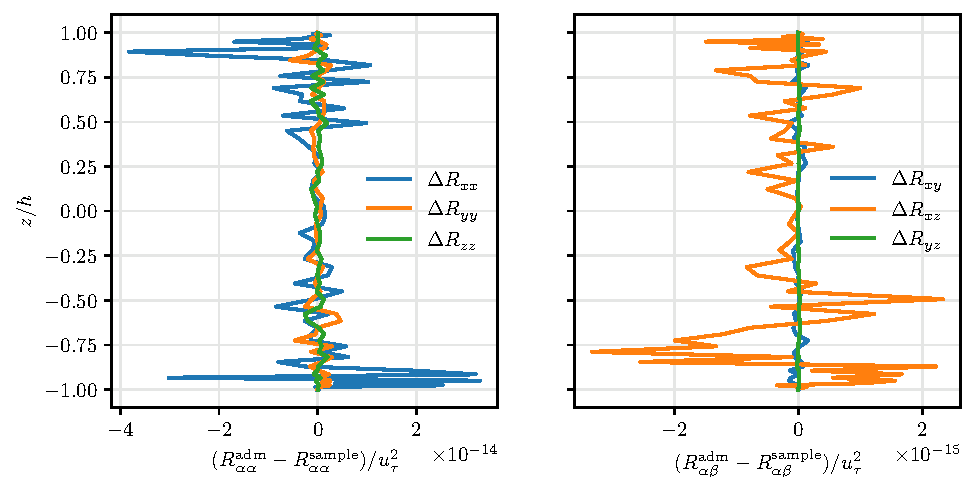
\includegraphics[width=0.95\linewidth]{figures/mkm_projected_reynolds_stress_errors.pdf}
  \caption{Pointwise differences between the Reynolds-stress profiles implied
  by \(\Badm\) and those sampled directly in physical space. The horizontal
  axes are nondimensionalized by \(u_{\tau}^2\). The errors are at roundoff
  level relative to the profile magnitudes.}
  \label{fig:projected_reynolds_errors}
\end{figure}

\section{Selected-mode channel resolvent analysis}
\label{sec:channel_resolvent_analysis}

The constraint construction in Section~\ref{sec:constraint} and the modal DNS
objects in Sections~\ref{sec:sampled_outputs} and
\ref{sec:projected_covariance} provide the ingredients needed for a
McKeon-style channel resolvent calculation. This section records the
implemented proof-of-concept framework. The implementation is selected-mode:
it computes the resolvent, DNS temporal cross-spectral density (CSD), DNS
projection fractions, and diagnostic figures for specified horizontal mode
indices. It is not yet an exhaustive mode sweep and should not be interpreted
as a high-Reynolds-number or long-box scaling result.

\subsection{Notation for a single horizontal mode}

Fix a horizontal Fourier mode with indices \((p,q)\), streamwise wavenumber
\(\kappa=\kappa_p\), and spanwise wavenumber \(\lambda=\lambda_q\). For this
mode the level-major velocity vector is
\begin{equation}
  \bfq
  =
  \begin{bmatrix}
    u_x(z_0) & u_y(z_0) & u_z(z_0) &
    \cdots &
    u_x(z_{N_z-1}) & u_y(z_{N_z-1}) & u_z(z_{N_z-1})
  \end{bmatrix}^{T}
  \in\mathbb{C}^{3N_z}.
  \label{eq:resolvent_level_major_vector}
\end{equation}
The component ordering in Eq.~\eqref{eq:resolvent_level_major_vector} is the
same ordering used by the target HDF5 file and by the constraint matrices:
streamwise, spanwise, wall-normal at each Chebyshev-Gauss level.

The turbulent mean profile is the streamwise component of the sampled mean,
\begin{equation}
  U_m = U(z_m) =
  \left(\texttt{mean\_profile}\right)_{m,0},
  \qquad m=0,\ldots,N_z-1.
  \label{eq:resolvent_mean_definition}
\end{equation}
The derivative matrix \(\Dz\) derived in Section~\ref{sec:constraint} gives
the discrete wall-normal mean shear
\begin{equation}
  U'_m = \left(\Dz U\right)_m.
  \label{eq:resolvent_mean_shear}
\end{equation}
All vectors and matrices below use the Chebyshev-Gauss physical quadrature
weights, not a uniform-grid approximation. Let \(w_m>0\) denote the Fejer
first-rule weights on \([-1,1]\), ordered consistently with \(z_m\). They are
defined by the quadrature rule
\begin{equation}
  \int_{-1}^{1} g(z)\,\dd z
  \approx
  \sum_{m=0}^{N_z-1} w_m g(z_m),
  \qquad
  \sum_{m=0}^{N_z-1} w_m \approx 2.
  \label{eq:resolvent_quadrature_rule}
\end{equation}
The implementation stores no kinetic-energy factor \(1/2\) in the weight. The
level-major velocity energy matrix is therefore
\begin{equation}
  W_q =
  \mathrm{diag}
  \left(
    w_0,w_0,w_0,\ldots,w_{N_z-1},w_{N_z-1},w_{N_z-1}
  \right).
  \label{eq:resolvent_wq_definition}
\end{equation}
For two modal velocity vectors \(\bfa,\bfb\in\mathbb{C}^{3N_z}\), the
implemented energy inner product is
\begin{equation}
  \langle \bfa,\bfb\rangle_{W_q}
  =
  \bfa^* W_q \bfb
  =
  \sum_{m=0}^{N_z-1} w_m
  \left[
    a_x(z_m)^* b_x(z_m)
    +a_y(z_m)^* b_y(z_m)
    +a_z(z_m)^* b_z(z_m)
  \right].
  \label{eq:resolvent_energy_inner_product}
\end{equation}

\subsection{Energy-orthonormal admissible basis}

For the chosen \((\kappa,\lambda)\), the compressed constraint matrix
\(\Gtilde(\kappa,\lambda)\) was derived in
Section~\ref{sec:constraint}. The admissible velocity subspace is
\begin{equation}
  \mathcal{V}_{\kappa,\lambda}
  =
  \left\{
    \bfq\in\mathbb{C}^{3N_z}:
    \Gtilde(\kappa,\lambda)\bfq=\bfzero
  \right\}.
  \label{eq:resolvent_admissible_subspace}
\end{equation}
The same singular-value convention used to construct \(\Gtilde\) also gives a
Euclidean null-space matrix \(N\), denoted \(\texttt{Nmat}\) in the code, such
that
\begin{equation}
  \Gtilde N = 0.
  \label{eq:resolvent_nullspace_property}
\end{equation}
The columns of \(N\) span the admissible space, but they are orthonormal in
the Euclidean inner product inherited from the SVD, not in the physical
quadrature energy inner product. The implemented resolvent instead needs a
matrix \(Q\) satisfying
\begin{equation}
  \Gtilde Q=0,
  \qquad
  Q^*W_qQ=I.
  \label{eq:resolvent_q_requirements}
\end{equation}
The construction is as follows. First form the Gram matrix
\begin{equation}
  M = N^*W_qN.
  \label{eq:resolvent_gram_matrix}
\end{equation}
Because \(W_q\) is positive diagonal and the columns of \(N\) are linearly
independent, \(M\) is Hermitian positive definite on the retained null space.
Let
\begin{equation}
  M = V\Lambda V^*
  \label{eq:resolvent_gram_eigendecomposition}
\end{equation}
be its Hermitian eigendecomposition, where
\(\Lambda=\mathrm{diag}(\mu_1,\ldots,\mu_r)\) with \(\mu_j>0\), and \(r\) is
the admissible dimension. Define
\begin{equation}
  Q = N V \Lambda^{-1/2}.
  \label{eq:resolvent_q_definition}
\end{equation}
Then the constraint property follows immediately from
Eq.~\eqref{eq:resolvent_nullspace_property}:
\begin{equation}
  \Gtilde Q
  =
  \Gtilde N V\Lambda^{-1/2}
  =
  0.
  \label{eq:resolvent_q_constraint_proof}
\end{equation}
The energy orthonormality follows by substituting
Eq.~\eqref{eq:resolvent_q_definition} into \(Q^*W_qQ\):
\begin{align}
  Q^*W_qQ
  &=
  \left(NV\Lambda^{-1/2}\right)^*
  W_q
  \left(NV\Lambda^{-1/2}\right) \nonumber\\
  &=
  \Lambda^{-1/2}V^*N^*W_qNV\Lambda^{-1/2}
  \nonumber\\
  &=
  \Lambda^{-1/2}V^*MV\Lambda^{-1/2}
  \nonumber\\
  &=
  \Lambda^{-1/2}\Lambda\Lambda^{-1/2}
  =
  I.
  \label{eq:resolvent_q_orthonormality_proof}
\end{align}
Consequently every admissible velocity vector represented by the reduced
coordinate vector \(\bfa\in\mathbb{C}^{r}\) has the form
\begin{equation}
  \bfq = Q\bfa,
  \label{eq:resolvent_q_reduced_coordinates}
\end{equation}
and its quadrature energy is
\begin{equation}
  \bfq^*W_q\bfq
  =
  \bfa^*Q^*W_qQ\bfa
  =
  \bfa^*\bfa.
  \label{eq:resolvent_reduced_energy}
\end{equation}
This identity is why the singular vectors of the reduced resolvent can be
mapped back to physical velocity space without any additional normalization.

\subsection{Pressure-eliminated velocity operator}

The velocity perturbation is written as a single Fourier harmonic,
\begin{equation}
  \bfu'(x,y,z,t)
  =
  \widehat{\bfu}(z,t)
  \exp\left[\ii(\kappa x+\lambda y)\right],
  \label{eq:resolvent_spatial_harmonic}
\end{equation}
and the mean velocity is \(U(z)\bm{e}_x\). Linearizing
Eq.~\eqref{eq:ns_momentum} around this mean gives
\begin{equation}
  \partial_t\bfu'
  =
  -U\partial_x\bfu'
  -u'_z U'\bm{e}_x
  -\nabla p'
  +
  \frac{1}{Re_{\tau}}\Delta\bfu'
  +
  \bff',
  \label{eq:resolvent_linearized_physical}
\end{equation}
where \(\bff'\) is a generic harmonic forcing representing the nonlinear
forcing residual in a resolvent interpretation. Equation
\eqref{eq:resolvent_linearized_physical} follows term by term from
\((U\bm{e}_x+\bfu')\cdot\nabla(U\bm{e}_x+\bfu')\): retaining only terms linear
in \(\bfu'\) gives \(U\partial_x\bfu'\) from advection of the perturbation by
the mean and \(u'_z U'\bm{e}_x\) from wall-normal displacement of the mean
profile.

Substituting the spatial harmonic in
Eq.~\eqref{eq:resolvent_spatial_harmonic} gives
\[
  \partial_x \mapsto \ii\kappa,\qquad
  \partial_y \mapsto \ii\lambda,\qquad
  \Delta \mapsto
  \partial_{zz}-(\kappa^2+\lambda^2).
\]
The wall-normal second derivative is represented by
\begin{equation}
  D_2=\Dz\Dz.
  \label{eq:resolvent_d2_definition}
\end{equation}
If \(\alpha^2=\kappa^2+\lambda^2\), the pressure-free part of the discrete
linearized velocity operator is therefore
\begin{equation}
  L_{\mathrm{raw}}\bfq
  =
  -\ii\kappa U\bfq
  -
  q_z U'\bm{e}_x
  +
  \frac{1}{Re_{\tau}}
  \left(D_2-\alpha^2 I\right)\bfq.
  \label{eq:resolvent_lraw_vector}
\end{equation}
The notation in Eq.~\eqref{eq:resolvent_lraw_vector} is level-major: the first
term multiplies all three velocity components at each \(z_m\) by
\(-\ii\kappa U_m\), the lift-up term adds \(-U'_m q_z(z_m)\) only to the
streamwise component, and the viscous scalar operator \(D_2-\alpha^2I\) is
applied independently to each velocity component.

The pressure term does no work against exactly divergence-free no-slip test
functions. In continuous form, if \(\bfv\) is incompressible and satisfies
\(\bfv=\bfzero\) at the walls and periodicity in \(x,y\), then
\begin{align}
  \int_{\Omega}\bfv^*\cdot\nabla p\,\dd\Omega
  &=
  \int_{\partial\Omega} p\,\bfv^*\cdot\bm{n}\,\dd S
  -
  \int_{\Omega}p\,\nabla\cdot\bfv^*\,\dd\Omega
  =
  0.
  \label{eq:resolvent_pressure_orthogonality}
\end{align}
The implemented proof of concept uses the corresponding velocity-only
admissible-subspace formulation: construct \(L_{\mathrm{raw}}\) from
Eq.~\eqref{eq:resolvent_lraw_vector}, restrict both trial and test vectors to
the columns of \(Q\), and form
\begin{equation}
  A = Q^*W_qL_{\mathrm{raw}}Q.
  \label{eq:resolvent_reduced_operator}
\end{equation}
The matrix \(A\in\mathbb{C}^{r\times r}\) is the reduced generator used by
the single-mode resolvent solver.

\subsection{Resolvent sign convention and singular modes}

Let \(\bfa(t)\) be the reduced velocity coordinate and let \(\bfb(t)\) be the
reduced forcing coordinate. With the projection above,
\begin{equation}
  \frac{\dd \bfa}{\dd t}=A\bfa+\bfb.
  \label{eq:resolvent_reduced_dynamics}
\end{equation}
The implemented Fourier-time convention is
\begin{equation}
  \bfa(t)=\widehat{\bfa}\exp(-\ii\omega t),
  \qquad
  \bfb(t)=\widehat{\bfb}\exp(-\ii\omega t).
  \label{eq:resolvent_time_harmonic}
\end{equation}
Substituting Eq.~\eqref{eq:resolvent_time_harmonic} into
Eq.~\eqref{eq:resolvent_reduced_dynamics} gives
\begin{equation}
  -\ii\omega\widehat{\bfa}
  =
  A\widehat{\bfa}+\widehat{\bfb}.
  \label{eq:resolvent_harmonic_balance}
\end{equation}
Moving the term \(A\widehat{\bfa}\) to the left gives
\begin{equation}
  \left(-\ii\omega I-A\right)\widehat{\bfa}
  =
  \widehat{\bfb}.
  \label{eq:resolvent_shifted_system}
\end{equation}
Thus the reduced resolvent matrix is
\begin{equation}
  H(\omega)
  =
  \left(-\ii\omega I-A\right)^{-1},
  \qquad
  \widehat{\bfa}=H(\omega)\widehat{\bfb}.
  \label{eq:resolvent_h_definition}
\end{equation}
The singular-value decomposition computed by the code is
\begin{equation}
  H(\omega)=\Psi(\omega)\Sigma(\omega)\Phi(\omega)^*,
  \label{eq:resolvent_svd}
\end{equation}
where the diagonal entries of \(\Sigma\) are nonnegative and sorted in
nonincreasing order. The reduced response modes are the columns of
\(\Psi\), and the reduced forcing modes are the columns of \(\Phi\). The
physical velocity modes written to HDF5 are
\begin{equation}
  \psi_j^{\mathrm{phys}} = Q\Psi_j,
  \qquad
  \phi_j^{\mathrm{phys}} = Q\Phi_j.
  \label{eq:resolvent_physical_modes}
\end{equation}
Because of Eq.~\eqref{eq:resolvent_q_orthonormality_proof} and the Euclidean
orthonormality of singular vectors, these physical modes satisfy
\begin{equation}
  \left(\psi_j^{\mathrm{phys}}\right)^*W_q\psi_k^{\mathrm{phys}}
  =
  \delta_{jk},
  \qquad
  \left(\phi_j^{\mathrm{phys}}\right)^*W_q\phi_k^{\mathrm{phys}}
  =
  \delta_{jk}.
  \label{eq:resolvent_physical_mode_normalization}
\end{equation}

The wall-normal energy-density diagnostic for a response mode is
\begin{equation}
  e_j(z_m;\omega)
  =
  \left|\psi_{j,x}^{\mathrm{phys}}(z_m;\omega)\right|^2
  +
  \left|\psi_{j,y}^{\mathrm{phys}}(z_m;\omega)\right|^2
  +
  \left|\psi_{j,z}^{\mathrm{phys}}(z_m;\omega)\right|^2.
  \label{eq:resolvent_energy_density}
\end{equation}
The component densities are the three terms in
Eq.~\eqref{eq:resolvent_energy_density}. The integrated mode energy is
\(\sum_m w_m e_j(z_m;\omega)\), which equals one up to roundoff for stored
response modes.

For \(\kappa\neq0\), the phase speed is
\begin{equation}
  c=\frac{\omega}{\kappa}.
  \label{eq:resolvent_phase_speed}
\end{equation}
Critical-layer locations are roots of
\begin{equation}
  U(z_c)=c.
  \label{eq:resolvent_critical_layer}
\end{equation}
The implementation sorts the Chebyshev-Gauss nodes by \(z\), searches for
sign changes in \(U(z)-c\), and linearly interpolates each crossing. If
\(\kappa=0\), Eq.~\eqref{eq:resolvent_phase_speed} has no finite phase speed,
so the critical-layer table is deliberately empty.

\subsection{Mode-resolved DNS temporal CSD}

For comparison with the resolvent response modes, the workflow estimates a
temporal CSD matrix for selected horizontal modes. For one selected mode, let
\(\bfq_n\in\mathbb{C}^{3N_z}\) be the modal DNS velocity fluctuation at
sample time \(t_n\). The series can come directly from the target dataset
\(\texttt{modal/u\_hat}\), or it can be computed on the fly from raw velocity
snapshots by subtracting the target mean profile and taking only the requested
horizontal Fourier coefficients.

If temporal demeaning is requested, the selected-record mean is removed before
segmentation:
\begin{equation}
  \bfq_n \leftarrow
  \bfq_n
  -
  \frac{1}{N_t}\sum_{\ell=0}^{N_t-1}\bfq_{\ell}.
  \label{eq:resolvent_temporal_demean}
\end{equation}
Let a segment have length \(L\), sample spacing \(\Delta t_s\), start index
\(s\), and temporal window \(g_n\), \(n=0,\ldots,L-1\). The unnormalized temporal
DFT used by \(\texttt{numpy.fft.fft}\) is
\begin{equation}
  \widehat{\bfq}^{(s)}_k
  =
  \sum_{n=0}^{L-1}
  g_n\bfq_{s+n}
  \exp\left(-2\pi\ii kn/L\right),
  \qquad k=0,\ldots,L-1.
  \label{eq:resolvent_csd_dft}
\end{equation}
The corresponding two-sided angular frequencies are
\begin{equation}
  \omega_k = 2\pi\,\mathrm{fftfreq}(L,\Delta t_s)_k,
  \label{eq:resolvent_csd_frequency_grid}
\end{equation}
and are stored sorted in ascending order. If there are \(N_{\mathrm{seg}}\)
segments and
\begin{equation}
  E_g=\sum_{n=0}^{L-1}g_n^2,
  \label{eq:resolvent_window_energy}
\end{equation}
then the implemented CSD estimator is
\begin{equation}
  S_{qq}(\omega_k)
  =
  \frac{\Delta t_s}{E_g N_{\mathrm{seg}}}
  \sum_{s=1}^{N_{\mathrm{seg}}}
  \widehat{\bfq}^{(s)}_k
  \left(\widehat{\bfq}^{(s)}_k\right)^*.
  \label{eq:resolvent_csd_estimator}
\end{equation}
This normalization is chosen so that Parseval's identity has the expected
weighted-energy form. With the unnormalized DFT in
Eq.~\eqref{eq:resolvent_csd_dft},
\begin{equation}
  \sum_{k=0}^{L-1}
  \left(\widehat{\bfq}^{(s)}_k\right)^*W_q
  \widehat{\bfq}^{(s)}_k
  =
  L\sum_{n=0}^{L-1}g_n^2\bfq_{s+n}^*W_q\bfq_{s+n}.
  \label{eq:resolvent_csd_parseval_dft}
\end{equation}
The frequency spacing is
\begin{equation}
  \Delta\omega=\frac{2\pi}{L\Delta t_s}.
  \label{eq:resolvent_csd_delta_omega}
\end{equation}
Using Eqs.~\eqref{eq:resolvent_csd_estimator} and
\eqref{eq:resolvent_csd_delta_omega},
\begin{align}
  \frac{1}{2\pi}
  \sum_{k=0}^{L-1}
  \mathrm{tr}\!\left(W_qS_{qq}(\omega_k)\right)
  \Delta\omega
  &=
  \frac{1}{2\pi}
  \sum_{k=0}^{L-1}
  \frac{\Delta t_s}{E_gN_{\mathrm{seg}}}
  \sum_s
  \left(\widehat{\bfq}^{(s)}_k\right)^*W_q
  \widehat{\bfq}^{(s)}_k
  \frac{2\pi}{L\Delta t_s}
  \nonumber\\
  &=
  \frac{1}{E_gN_{\mathrm{seg}}}
  \sum_s
  \frac{1}{L}
  \sum_{k=0}^{L-1}
  \left(\widehat{\bfq}^{(s)}_k\right)^*W_q
  \widehat{\bfq}^{(s)}_k
  \nonumber\\
  &=
  \frac{1}{E_gN_{\mathrm{seg}}}
  \sum_s
  \sum_{n=0}^{L-1}
  g_n^2\bfq_{s+n}^*W_q\bfq_{s+n}.
  \label{eq:resolvent_csd_parseval_result}
\end{align}
Thus the integrated CSD energy equals the window-weighted segment-average
modal energy. For a rectangular window and one full-record segment, this is
the ordinary selected-record time-mean modal energy. For Hann-windowed,
overlapping production estimates, Eq.~\eqref{eq:resolvent_csd_parseval_result}
is still the diagnostic being checked, but it is a window-weighted
segment-average identity rather than an unwindowed whole-record variance.

\subsection{Projection of DNS CSD onto response modes}

At a frequency where both the resolvent and DNS CSD are available, let
\[
  \Psi_r =
  \begin{bmatrix}
  \psi_1^{\mathrm{phys}} & \cdots & \psi_r^{\mathrm{phys}}
  \end{bmatrix}
  \in\mathbb{C}^{3N_z\times r}
\]
be the first \(r\) stored response modes. The columns satisfy
\(\Psi_r^*W_q\Psi_r=I_r\). The total DNS spectral energy at that frequency is
\begin{equation}
  E_{\mathrm{DNS}}(\omega)
  =
  \mathrm{tr}\!\left(W_qS_{qq}(\omega)\right).
  \label{eq:resolvent_projection_total_energy}
\end{equation}
The response-basis coefficient matrix is
\begin{equation}
  C_r(\omega)
  =
  \Psi_r^*W_qS_{qq}(\omega)W_q\Psi_r.
  \label{eq:resolvent_projection_coefficients}
\end{equation}
To see why Eq.~\eqref{eq:resolvent_projection_coefficients} is the correct
coefficient matrix, define the rank-\(r\) CSD reconstruction
\begin{equation}
  S_r(\omega)=\Psi_r C_r(\omega)\Psi_r^*.
  \label{eq:resolvent_projection_reconstruction}
\end{equation}
Taking its weighted trace and using cyclic invariance gives
\begin{align}
  \mathrm{tr}\!\left(W_qS_r\right)
  &=
  \mathrm{tr}\!\left(W_q\Psi_r C_r\Psi_r^*\right)
  =
  \mathrm{tr}\!\left(\Psi_r^*W_q\Psi_r C_r\right)
  =
  \mathrm{tr}\!\left(C_r\right),
  \label{eq:resolvent_projection_energy_trace}
\end{align}
because \(\Psi_r^*W_q\Psi_r=I_r\). Therefore the DNS energy associated with
the \(j\)-th response direction is the \(j\)-th diagonal entry of \(C_r\):
\begin{equation}
  E_j(\omega)
  =
  \left(C_r(\omega)\right)_{jj}
  =
  \left(\psi_j^{\mathrm{phys}}\right)^*
  W_qS_{qq}(\omega)W_q
  \psi_j^{\mathrm{phys}}.
  \label{eq:resolvent_projection_single_energy}
\end{equation}
The rank-one and cumulative rank-\(r\) fractions reported by the code are
\begin{equation}
  F_j(\omega)
  =
  \frac{\mathrm{Re}\,E_j(\omega)}
       {E_{\mathrm{DNS}}(\omega)},
  \qquad
  F_{\le r}(\omega)
  =
  \frac{\mathrm{Re}\,\mathrm{tr}\,C_r(\omega)}
       {E_{\mathrm{DNS}}(\omega)}.
  \label{eq:resolvent_projection_fractions}
\end{equation}
The implementation also reports the weighted Frobenius relative error of
Eq.~\eqref{eq:resolvent_projection_reconstruction},
\begin{equation}
  \epsilon_r(\omega)
  =
  \frac{
  \left\|
    W_q^{1/2}\left[S_{qq}(\omega)-S_r(\omega)\right]W_q^{1/2}
  \right\|_F}
  {
  \left\|
    W_q^{1/2}S_{qq}(\omega)W_q^{1/2}
  \right\|_F}.
  \label{eq:resolvent_projection_frobenius_error}
\end{equation}
Before projection, frequencies are matched exactly to the selected CSD grid
within a prescribed tolerance; a mismatch is treated as an error rather than
interpolated silently.

\subsection{Implemented scripts and HDF5 outputs}

The framework is implemented by the scripts listed in
Table~\ref{tab:resolvent_implemented_scripts}.

\begin{table}[H]
  \centering
  \caption{Main scripts in the selected-mode channel-resolvent workflow.}
  \label{tab:resolvent_implemented_scripts}
  \begin{tabular}{p{0.44\linewidth}p{0.48\linewidth}}
    \toprule
    Script & Role \\
    \midrule
    \path{mkm_channel_resolvent_utils.py}
      & Shared constraints, weights, bases, operators, and diagnostics. \\
    \path{compute_mkm_channel_resolvent.py}
      & Single-mode resolvent HDF5 writer. \\
    \path{plot_mkm_channel_resolvent.py}
      & Mode-shape, gain, critical-layer, and reconstructed-field PDFs. \\
    \path{compute_mkm_modal_csd.py}
      & Selected-mode temporal DNS CSD estimator. \\
    \path{project_mkm_dns_onto_resolvent.py}
      & DNS CSD projection fractions. \\
    \path{run_mkm_channel_resolvent_selected_modes.py}
      & Selected-mode workflow driver. \\
    \path{run_mkm_channel_resolvent_production_selected_modes.py}
      & Production wrapper with server paths and missing-file checks. \\
    \path{report_mkm_channel_resolvent_workflow.py}
      & Markdown audit report generator. \\
    \bottomrule
  \end{tabular}
\end{table}
The single-mode resolvent HDF5 file contains the groups in
Table~\ref{tab:resolvent_hdf5_schema}. The CSD and projection files contain
the groups in Tables~\ref{tab:csd_hdf5_schema} and
\ref{tab:projection_hdf5_schema}.

\begin{table}[H]
  \centering
  \caption{Main HDF5 datasets written by the single-mode resolvent solver.}
  \label{tab:resolvent_hdf5_schema}
  \begin{tabular}{p{0.36\linewidth}p{0.56\linewidth}}
    \toprule
    Dataset & Meaning \\
    \midrule
    \path{geometry/z_wall}, \path{geometry/k_stream}, \path{geometry/k_span}
      & Wall-normal grid and horizontal wavenumber arrays. \\
    \path{mean/U}, \path{mean/Uprime}
      & Turbulent mean profile and \(U'=\Dz U\). \\
    \path{mode/index}, \path{mode/kappa}, \path{mode/lambda}
      & Selected mode indices and physical wavenumbers. \\
    \path{frequencies/omega}
      & Stored angular frequencies. \\
    \path{critical_layers/z},
    \path{critical_layers/y_plus_nearest_wall},
    \path{critical_layers/count}
      & Roots of \(U(z)=\omega/\kappa\), corresponding nearest-wall
      \(y^+\), and root counts. \\
    \path{resolvent/singular_values}
      & Diagonal entries of \(\Sigma(\omega)\). \\
    \path{resolvent/response_modes},
    \path{resolvent/forcing_modes}
      & \(W_q\)-normalized physical modes \(Q\Psi_j\) and \(Q\Phi_j\). \\
    \path{resolvent/response_energy_density},
    \path{resolvent/component_energy_density}
      & Unweighted pointwise densities
      \(e_j(z_m)\) and component contributions. \\
    \path{diagnostics/*}
      & Constraint residuals, energy-norm errors, basis
      orthonormality error, resolvent condition numbers, and constraint
      singular values. \\
    \bottomrule
  \end{tabular}
\end{table}

\begin{table}[H]
  \centering
  \caption{Main HDF5 datasets written by the selected-mode CSD estimator.}
  \label{tab:csd_hdf5_schema}
  \begin{tabular}{p{0.36\linewidth}p{0.56\linewidth}}
    \toprule
    Dataset & Meaning \\
    \midrule
    \path{mode/index}, \path{mode/k_stream}, \path{mode/k_span}
      & Selected mode rows and physical wavenumbers. \\
    \path{frequencies/omega}
      & Sorted two-sided angular frequency grid. \\
    \path{csd/Sqq}
      & \(S_{qq}\), shape
      \((N_{\mathrm{mode}},N_{\omega},3N_z,3N_z)\). \\
    \path{csd/trace}
      & Ordinary matrix trace of \(S_{qq}\). \\
    \path{csd/component_trace}
      & Wall-normal-weighted component energy spectra. \\
    \path{csd/energy_trace}
      & \(\mathrm{tr}(W_qS_{qq})\). \\
    \path{metadata/*}
      & Selected times, snapshot keys, window, window energy, sample
      spacing, segment length, overlap, source, and demeaning flag. \\
    \path{diagnostics/parseval_energy_time},
    \path{diagnostics/parseval_energy_spectrum},
    \path{diagnostics/parseval_relative_error}
      & The two sides of Eq.~\eqref{eq:resolvent_csd_parseval_result} and
      their relative difference. \\
    \bottomrule
  \end{tabular}
\end{table}

\begin{table}[H]
  \centering
  \caption{Main HDF5 datasets written by the DNS-to-resolvent projection.}
  \label{tab:projection_hdf5_schema}
  \begin{tabular}{p{0.36\linewidth}p{0.56\linewidth}}
    \toprule
    Dataset & Meaning \\
    \midrule
    \path{mode/index}, \path{mode/k_stream}, \path{mode/k_span}
      & Matched single resolvent mode. \\
    \path{frequencies/resolvent_omega},
    \path{frequencies/csd_omega},
    \path{frequencies/csd_index}
      & Resolvent frequencies, matched CSD frequencies, and CSD grid
      indices. \\
    \path{projection/energy_total}
      & \(E_{\mathrm{DNS}}=\mathrm{tr}(W_qS_{qq})\). \\
    \path{projection/energy_fraction}
      & \(F_j\) in Eq.~\eqref{eq:resolvent_projection_fractions}. \\
    \path{projection/cumulative_energy_fraction}
      & \(F_{\le r}\) for ranks \(1,\ldots,r_{\max}\). \\
    \path{projection/modal_coefficients}
      & \(C_r=\Psi_r^*W_qS_{qq}W_q\Psi_r\). \\
    \path{projection/weighted_frobenius_relative_error}
      & \(\epsilon_r\) from
      Eq.~\eqref{eq:resolvent_projection_frobenius_error}. \\
    \path{diagnostics/*}
      & Frequency match errors, mode match error, response norm errors,
      and negative-fraction counts. \\
    \bottomrule
  \end{tabular}
\end{table}

The plotting script reads the physical response and forcing modes and writes
four PDFs for each selected mode:
\begin{equation}
\begin{aligned}
  &\texttt{mkm\_resolvent\_mode\_shapes.pdf},\\
  &\texttt{mkm\_resolvent\_gain\_bode.pdf},\\
  &\texttt{mkm\_resolvent\_peak\_location\_gain.pdf},\\
  &\texttt{mkm\_resolvent\_reconstructed\_fields.pdf}.
\end{aligned}
\label{eq:resolvent_pdf_outputs}
\end{equation}
The reconstructed fields use
\begin{equation}
  u_{\alpha}^{\mathrm{real}}(x,y,z)
  =
  \mathrm{Re}
  \left[
    \psi_{\alpha}(z)
    \exp\left(\ii(\kappa x+\lambda y+\varphi)\right)
  \right],
  \qquad \alpha\in\{x,y,z\},
  \label{eq:resolvent_reconstructed_field}
\end{equation}
where \(\varphi\) is the requested plotting phase.

\subsection{Production selected-mode runs}

Two production selected-mode workflows have been completed. Both used the
production target
\begin{center}
  \path{/media/jay/data1/shenfun_dns_runs/production_mkm_64_64_32_20260702/MKM_production_64_64_32_target_t60_t180.h5}
\end{center}
and the matching Chebyshev/quadrature constraint file. The selected modes were
\begin{equation}
  (p,q)=(1,0),\qquad (1,1),\qquad (2,1).
  \label{eq:resolvent_selected_modes}
\end{equation}
Since \(L_x=2\pi\) and \(L_y=\pi\), these correspond to
\[
  (\kappa,\lambda)=(1,0),\qquad (1,2),\qquad (2,2).
\]
The sparse target-CSD run used the stored target \(\texttt{modal/u\_hat}\)
series. The dense temporal-CSD run used selected horizontal modes computed
from the dense raw velocity continuation. Table~\ref{tab:resolvent_csd_sources}
summarizes the two CSD sources.

\begin{table}[H]
  \centering
  \caption{CSD sources used in the completed production selected-mode
  resolvent workflows.}
  \label{tab:resolvent_csd_sources}
  \small
  \begin{tabular}{p{0.18\linewidth}p{0.20\linewidth}p{0.16\linewidth}ccc}
    \toprule
    Run & Source & Record & \(\Delta t_s\) & Segment length & Segments \\
    \midrule
    Sparse target CSD
      & \(\texttt{modal/u\_hat}\)
      & \(60\le t\le180\)
      & \(0.1\)
      & \(512\)
      & \(3\) \\
    Dense temporal CSD
      & raw selected FFT modes
      & \(180\le t\le300\)
      & \(0.01\)
      & \(2048\)
      & \(10\) \\
    \bottomrule
  \end{tabular}
\end{table}

Both production CSD estimates used a Hann window and selected-record temporal
demeaning. The sparse target run used the first four positive CSD bins,
\begin{equation}
  \omega =
  0.122718,\;0.245437,\;0.368155,\;0.490874,
  \label{eq:resolvent_sparse_omega}
\end{equation}
while the dense temporal run used the first six positive dense-CSD bins,
\begin{equation}
  \omega =
  0.306796,\;0.613592,\;0.920388,\;1.227185,\;1.533981,\;1.840777.
  \label{eq:resolvent_dense_omega}
\end{equation}
The two frequency grids are different; the comparison below should therefore
be read as a trend and infrastructure check, not as a pointwise same-frequency
comparison.

Table~\ref{tab:resolvent_sparse_results} gives the sparse target-CSD results.
Table~\ref{tab:resolvent_dense_results} gives the dense temporal-CSD results.
The gain range is the range of the leading singular value over the stored
frequencies. The projection columns report the maximum rank-one fraction
\(F_1\) and the maximum cumulative rank-six fraction \(F_{\le6}\) over the
stored frequencies.

\begin{table}[H]
  \centering
  \caption{Sparse target-CSD selected-mode resolvent results.}
  \label{tab:resolvent_sparse_results}
  \begin{tabular}{lcccc}
    \toprule
    Mode & \((\kappa,\lambda)\) & Leading gain range
      & \(\max F_1\) & \(\max F_{\le6}\) \\
    \midrule
    \((1,0)\) & \((1,0)\) & \(0.145890\)--\(0.152295\)
      & \(0.123227\) at \(\omega=0.368155\)
      & \(0.407893\) at \(\omega=0.368155\) \\
    \((1,1)\) & \((1,2)\) & \(0.183654\)--\(0.193115\)
      & \(0.161356\) at \(\omega=0.245437\)
      & \(0.490194\) at \(\omega=0.368155\) \\
    \((2,1)\) & \((2,2)\) & \(0.092078\)--\(0.094563\)
      & \(0.059074\) at \(\omega=0.245437\)
      & \(0.265905\) at \(\omega=0.368155\) \\
    \bottomrule
  \end{tabular}
\end{table}

\begin{table}[H]
  \centering
  \caption{Dense temporal-CSD selected-mode resolvent results.}
  \label{tab:resolvent_dense_results}
  \begin{tabular}{lcccc}
    \toprule
    Mode & \((\kappa,\lambda)\) & Leading gain range
      & \(\max F_1\) & \(\max F_{\le6}\) \\
    \midrule
    \((1,0)\) & \((1,0)\) & \(0.149034\)--\(0.180371\)
      & \(0.115051\) at \(\omega=0.613592\)
      & \(0.335164\) at \(\omega=0.613592\) \\
    \((1,1)\) & \((1,2)\) & \(0.188284\)--\(0.235934\)
      & \(0.219378\) at \(\omega=0.306796\)
      & \(0.422372\) at \(\omega=0.306796\) \\
    \((2,1)\) & \((2,2)\) & \(0.093306\)--\(0.104738\)
      & \(0.082318\) at \(\omega=0.613592\)
      & \(0.356971\) at \(\omega=0.613592\) \\
    \bottomrule
  \end{tabular}
\end{table}

Across these selected low-wavenumber modes, mode \((1,1)\), corresponding to
\((\kappa,\lambda)=(1,2)\), is the most consistently aligned with the leading
response mode. The dense temporal estimate raises its maximum rank-one
projection fraction from approximately \(16\%\) in the sparse target-CSD run
to approximately \(22\%\). Rank six captures a substantially larger fraction
than rank one: about \(22\%\)--\(49\%\) in the sparse target-CSD run and about
\(26\%\)--\(42\%\) in the dense temporal-CSD run over these modes and
frequencies. A low rank-one fraction does not invalidate the resolvent model;
it can reflect forcing statistics not aligned with the leading forcing mode,
finite response rank, low Reynolds number, the short streamwise box, selected
frequency bins that are not centered on the most energetic CSD bands, and
finite-sample CSD estimation.

The numerical diagnostics are near roundoff. The maximum CSD Parseval relative
errors were \(2.93\times10^{-15}\) for the sparse target-CSD run and
\(6.17\times10^{-15}\) for the dense temporal-CSD run. Across the resolvent
outputs, the largest response and forcing constraint residuals were below
\(5\times10^{-15}\), the largest response and forcing energy-normalization
errors were below \(4\times10^{-15}\), and the projection frequency-match
errors were zero for the stored frequencies.

\subsection{Representative generated figures}

The workflow wrote a complete four-PDF figure set for every selected mode in
both the sparse and dense production directories. The local lightweight
artifacts are under
\begin{center}
  \path{scripts/mkm_dns_target/production_reports/target_csd_selected_modes/}
\end{center}
and
\begin{center}
  \path{scripts/mkm_dns_target/production_reports/dense_csd_selected_modes/}.
\end{center}
The large HDF5 products remain on the Linux server and were intentionally not
copied into the repository.

Figures~\ref{fig:resolvent_target_i1j1} and
\ref{fig:resolvent_dense_i1j1} show the representative mode \((1,1)\), the
mode with the strongest leading-response alignment in the comparison above.
The mode-shape panels plot \(|u_x|\), \(|u_y|\), and \(|u_z|\) versus \(z/h\)
for the stored response and forcing modes at the selected frequency index.
The gain panels plot the singular values versus \(\omega\). The peak-location
panels compare the wall-normal location of maximum leading-response energy
with stored critical-layer roots. The reconstructed-field panels show real
physical velocity slices computed from
Eq.~\eqref{eq:resolvent_reconstructed_field}.

\begin{figure}[H]
  \centering
  \begin{minipage}{0.48\linewidth}
    \centering
    
\includegraphics[width=\linewidth]{../production_reports/target_csd_selected_modes/figures_i1_j1/mkm_resolvent_mode_shapes.pdf}\\
    \small Mode shapes
  \end{minipage}\hfill
  \begin{minipage}{0.48\linewidth}
    \centering
    
\includegraphics[width=\linewidth]{../production_reports/target_csd_selected_modes/figures_i1_j1/mkm_resolvent_gain_bode.pdf}\\
    \small Singular-value gain curves
  \end{minipage}

  \vspace{0.8em}

  \begin{minipage}{0.48\linewidth}
    \centering
    
\includegraphics[width=\linewidth]{../production_reports/target_csd_selected_modes/figures_i1_j1/mkm_resolvent_peak_location_gain.pdf}\\
    \small Peak energy and critical layer
  \end{minipage}\hfill
  \begin{minipage}{0.48\linewidth}
    \centering
    
\includegraphics[width=\linewidth]{../production_reports/target_csd_selected_modes/figures_i1_j1/mkm_resolvent_reconstructed_fields.pdf}\\
    \small Reconstructed physical fields
  \end{minipage}
  \caption{Sparse target-CSD selected-mode resolvent figures for mode
  \((1,1)\), corresponding to \((\kappa,\lambda)=(1,2)\).}
  \label{fig:resolvent_target_i1j1}
\end{figure}

\begin{figure}[H]
  \centering
  \begin{minipage}{0.48\linewidth}
    \centering
    
\includegraphics[width=\linewidth]{../production_reports/dense_csd_selected_modes/figures_i1_j1/mkm_resolvent_mode_shapes.pdf}\\
    \small Mode shapes
  \end{minipage}\hfill
  \begin{minipage}{0.48\linewidth}
    \centering
    
\includegraphics[width=\linewidth]{../production_reports/dense_csd_selected_modes/figures_i1_j1/mkm_resolvent_gain_bode.pdf}\\
    \small Singular-value gain curves
  \end{minipage}

  \vspace{0.8em}

  \begin{minipage}{0.48\linewidth}
    \centering
    
\includegraphics[width=\linewidth]{../production_reports/dense_csd_selected_modes/figures_i1_j1/mkm_resolvent_peak_location_gain.pdf}\\
    \small Peak energy and critical layer
  \end{minipage}\hfill
  \begin{minipage}{0.48\linewidth}
    \centering
    
\includegraphics[width=\linewidth]{../production_reports/dense_csd_selected_modes/figures_i1_j1/mkm_resolvent_reconstructed_fields.pdf}\\
    \small Reconstructed physical fields
  \end{minipage}
  \caption{Dense temporal-CSD selected-mode resolvent figures for mode
  \((1,1)\), corresponding to \((\kappa,\lambda)=(1,2)\).}
  \label{fig:resolvent_dense_i1j1}
\end{figure}

The complete local figure set includes the same four PDFs for modes
\((1,0)\), \((1,1)\), and \((2,1)\) in both CSD-source directories. The
workflow manifest JSON files record the exact HDF5 paths, frequencies,
leading singular values, constraint residuals, projection fractions, and
figure paths. The generated Markdown reports summarize those manifests and
serve as compact audit records for future production reruns.

\section{Reproducibility remarks}

The production handoff file
\[
  \texttt{HANDOFF\_production\_mkm\_64\_64\_32.md}
\]
records the exact server paths, commands, convergence reports, and audit
files. For future runs on this mesh, the validated production setting is
16 MPI ranks. A different MPI decomposition should be re-tested together with
the FFT pencil decomposition constraints. If a stricter scalar-energy
stationarity criterion is required, the sampling record should be extended
beyond \(t u_{\tau}/h=180\), and the retained-window field and scalar
convergence checks should be repeated before regenerating the target
covariance.

\end{document}
